	\chapter{C} \label{c_crash} 

Many people who use a computer to do statistics and simulations never
took a computer science course. They jumped in and started writing
using the scripting language associated with their favorite statistics or
symbolic math package. This is truly the ideal way to start out with writing
code, but as the code becomes a bigger part of their lives---when the
dissertation relies on computer code---it is worth pausing to consider
code-writing in more detail. 

This chapter takes the next step, introducing C and some of the
concepts behind good programming that script-writers often overlook.
I will cover both the syntax of C and many concepts that are in no way
C-specific. The functional approach, stacks of frames, debugging,
test functions, and overall good style are immediately applicable to
virtually every programming language in use today.\footnote{What does
change from language to language?  Besides the details of syntax, the
rules for scope and the call-by-value/call-by-reference mechanism tend
to be different for every language. When faced with a new language, I
always check the scoping rules first.} Thus, this chapter on C may help
the reader to become a better programmer with any programming language.

As for the syntax of C, this chapter will cover only a subset. C has
32 key words and this book will only use 18 of them.\footnote{For
comparison, C$^{++}$ has 49 key words, and  Java has an even 50.} Some of the other keywords are basically
archaic, designed for the days when compilers needed help from the user to
optimize code. Others, like bit-shifting operators, are only useful
if you are writing an operating system or a hardware device driver. With
all the parts of C that directly manipulate hexadecimal memory addresses
omitted, you will find that at its core, C is a rather simple language
that is perfectly designed for simulations and handling large data sets.
If you really do want to know about bit-shifting operators, just type
\bi{C tutorial} into your favorite search engine; since this is C and
not a proprietary, specialized language, you will have a few hundred
hits to choose from.
\comment{
Finally, don't feel compelled to memorize everything here (using
\ci{malloc} three times in a sentence, for example), since this book and
the online references are always there for you to read. The best way to
learn the details is to sit down at a computer and write. 
}

\paragraph{An outline} 

This chapter divides into three parts.  Sections \ref{fncontents} and
\ref{declaring} start small, covering the syntax of individual lines
of code to make assignments, do arithmetic, and declare variables.
Sections \ref{functional} and \ref{compilation} introduce functions,
describing how C is built on the idea of modular functions that are each
independently built and evaluated.  Sections \ref{pointers} through
\ref{stringsec} cover \airq{pointers}, a C-specific means of handling
computer memory that complements C's means of handling functions and
large data structures. The remainder of the chapter covers the art of
debugging code, and some tips on writing bug-free code to begin with. 

\subsection{The tools} 
Most stats packages are built around a single window that includes a
space for you to type commands and a space for output to be displayed.
They also give you the option of putting all of your commands into a
text file, and then the package reads the text file and displays output.

First, C works almost entirely in the paradigm of putting commands in a
text file and then running the text file all at once. Second, since
C is an open standard rather than a product from a single company or
foundation, there
are hundreds of programs available to help you write the text file and
produce the output. Your problem is not in finding such tools, but in
choosing which you will use.

The first element you will need is a compiler. If you are using
a UNIX-like system, you probably already have \cind{gcc} on your
computer. Try typing \bi{cc} on your command line; if you get an
error like ``command not found'', then you will need to get a compiler,
but an error like ``no input files'' means that a compiler was found
and awaits input. Windows and MacOS do not ship with a compiler, but if you
are using a computer customized by your university or company computing
department, check the usual application folders.

On top of the compiler, you will need a debugger like gdb, the standard
libraries, the GNU Scientific Library (GSL) and SQLite.  The easiest way
to get all of these disparate tools is via a package manager. With a
package manager, the installation process is short; without one,
the process is nasty and brutish.

If you are using a UNIX-like system, you are probably already familiar
with your package manager (Red Hat Package Manager and Debian's Apt are
the most popular).

If you are using Windows, you have two options. One is to get
Mingw, which provides a compiler and some basic auxiliary tools. It has its
own installation program and some package facilities. The other option is to
get Cygwin.  It is free, has a pleasant package-oriented installation
program, and provides an entire UNIX subsystem, with the attendant
compilers, editors, and so on. Be sure to select gcc, gdb, the GSL,
and SQLite under the development subsection in the installation.

Mac OS X users will be using the terminal (typically found in the
accessories subfolder of the applications folder) to do
most of the work below. The package manager of choice is Fink, which
can easily be found and installed online.

Herein, I will assume that you have a working copy of \ci{gcc},
\ci{gdb}, et cetera, and it is on the search path for executables
on your system. If this is not the case, then abundant help is available,
either from your local computer guru or from your favorite search engine.

If you will be using Apophenia or would like further notes on
installation, see the Setup section of the online reference, at
\onlinereflocation.

\paragraph{IDEs} \index{IDE} \index{integrated development environment}
Broadly, you have the choice of two paradigms in which to work. The
first is the integrated development environment (IDE). This is an
all-in-one environment comparable to a multiwindow stats package, with
one window for your program, one for compilation, one for output, et
cetera.  
Popular choices include Dev-C++ or Eclipse. Many other IDEs of varying
quality are available for any graphically-oriented operating system.

The other option is via the command line. Since you are certainly using
a system that supports multiple windows,\footnote{Even if you are
dialing in to a server's single-window terminal, you can either dial in
twice, or use \bi{screen} to multiplex the window.} 
you are basically using your operating system as an IDE.
In this paradigm, you will probably have one window that is dedicated to
a text editor with your code, and another window or two for compilation,
debugging, and output.


\exercise{Check your C environment by compiling and running 
``Hello, world,'' a classic first program adapted from \citet{kandr:c}. 
\begin{itemize}
\itemsep 0pt
\item Download the sample code for this book from \samplecodelocation.
\item Decompress the \bi{.zip} file, go into the directory thus created, and compile the
program with the command \bi{gcc hello\_world.c}. If you are using an
IDE, see your manual for compilation instructions.
\end{itemize}
(continued)
}
\exercise{(continued)
\begin{itemize}
\item If all went well, you will now have a program in the directory
named \bi{a.out}. From the command line, you can execute it using
\bi{./a.out}.
\item If that basic compilation went well, you may also want to try the
\bi{Makefile} included the \bi{.zip} file. See the instructions in the
file.
\end{itemize}

If you have trouble, see the setup notes at \onlinereflocation{} for
troubleshooting notes, or copy and paste the error message into your
favorite search engine.}


\paragraph{Text files} C programs are files of text, and all of your work
will be manipulations of text, so it is in your long-run best interest to
get a good \ind{text editor}. At the very least, you will get error messages
listing line numbers, so if your text editor can't tell you which is
line 105, you will need to get a new one.

The two most popular are \ind{EMACS} and \ind{vi}. EMACS is better for
people who prefer to have everything under one roof---it is often billed
as an IDE---while vi is better for the minimalists and touch typists. Both
involve a learning curve, meaning that they will be difficult to use at
first, will require reading the manual, and will in the long run save
you hours over using simpler text editors such as those typically
included with IDEs. Some implementation of both is available for all
computer types, and you are encouraged to start learning one or the other
now. If neither suits your fancy, there are literally hundreds of others
to choose from. That said, I will assume you have a good text editor
(by your personal definition of \airq{good}), and will turn to the text you
will be writing with it.

\comment{
\subsection{An opening sample}
To get the conversation started, here is a complete sample program.
The program writes down a vector of numbers, and prints their mean.
\label{initialsample}
\begin{lstlisting}[numbers=left, numberstyle=\scshape]
#include <stdio.h>

int main(void){
    float data[] = {2,4,8,16,32};
    int data_ct = 5;
    int i;
    float mean = 0;
    for (i=0; i< data_ct; i++){
        mean += data[i];
    }
    mean /= data_ct;
    printf("The mean is %g.\n", avg);
    return 0;
}
\end{lstlisting}
Line 1 is a call to an external header file, and will
be discussed in Section \ref{headers}. 

Line 3 is a function header. A C program does only two things: allocate
variables and run functions.  You will see time and time again that the
focus in writing good code is not about writing out lengthy procedures, but 
writing small functions that do one thing well. The entire program as
such is just a function named \ci{main}. Since functions typically
output a value, and line 13 shows that this function returns zero.

Inside this function, the first thing we do is allocate variables. As in
Section \ref{declaring}, all variables have to be declared. Line four
declares an array of five data points, and lines 5--7 declare scalars.

Lines 8--10 are a \ci{for} loop. Line 8 may seem ornery, but
Section \ref{forloops} will explain that it simply takes the variable
\ci{i} through the indices of the \ci{data} vector. 

Line 9 increments  the value of \ci{avg} by the value of the
\ci{i}th element of the \ci{data} array. In R, this would be
written as \ci{mean <- mean + data[i]}, and similarly in other
languages. 

By line 11, \ci{mean} has the sum of all of the elements of the
vector, and line 11 divides the mean by the number of data points to
produce the actual mean. 

Some stats packages print out every step of the process; C is much
quieter and will only speak when asked.  Line 12 actually prints out
the value of the mean. Its syntax is explained on page \pageref{printf}.

If you are familiar with the commands of the typical stats package, the
program should have some familiar and unfamiliar components. The odd
syntax, such as the line about the \ci{for} loop, is simply a
question of getting used to a new language. For many scriptwriters,
the fact that everything happens in the context of a function is often
a new means of thinking about writing a program. It is not the most
direct means, but by the end of this chapter you should see its immense
benefit. The variable declarations may be a bit tedious, but they are
easy enough.
}

\section{Lines} \label{fncontents}

The story begins at the smallest level: a single line of code. Most of
the work on a single line of code will be familiar to anyone who has
written programs in any language, including instructions like assignments,
basic arithmetic, if-then conditions, and loops. For such common
programming elements, learning C is simply a question of the details
of syntax. Also, C is a \airq{typed} language, meaning that you will
need to specify whether every variable and function is an integer,
a real, a vector, et cetera. Thus, many of the lines will be simple
type declarations.

\subsection{Assignment} \index{arithmetic} \index{assignment|see{=}} \index{=}
Most of the work you will be doing will be simple assignments. For example,
\begin{lstlisting}
ratio = a / b;
\end{lstlisting}
will find the value of \ci{a} divided by \ci{b} and put the
value in \ci{ratio}. Notice that there is a semicolon at the end of
the line; you will need a semicolon at the end of everything but the few
exceptions I mention below.\footnote{The number one cause of compiler
complaints like ``line 41: \ind{syntax error}'' is a missing semicolon on line 40.} All of the usual operations work: \ci{+
- / *}, and so do some of the more obscure ones, like \ci{a \% b}
for $a$ mod $b$. \index{modulo|see{\%}} \index{\%}

\subsection{Incrementing}\index{incrementing} It is incredibly common to have an operation of the form \ci{a = a + b;}---so
common that C has a special syntax for it: \ci{a += b;} This is slightly less readable, but involves less
redundancy. All of the above arithmetic operators can take this form, so each of the following lines show two
equivalent expressions: \\


\ns{5}
\begin{lstlisting}
a -= b;  /*is equivalent to*/   a = a - b;
a *= b;  /*is equivalent to*/   a = a * b;
a /= b;  /*is equivalent to*/   a = a / b;
a %= b;  /*is equivalent to*/   a = a % b;
\end{lstlisting}

Finally, the most common operation among these is incrementing or decrementing by one, and so C offers the
following syntax for still less typing:\footnote{There is also the pre-increment form, \ci{++a} and
\ci{--a}. Pre- and post-incrementing differ only when they are being used in situations that are bad style and should
be avoided. Leave these operations on a separate line and stick to whichever form looks nicer to you.} \\
\begin{lstlisting}
a++; /*is equivalent to*/ a = a + 1;
a--; /*is equivalent to*/ a = a - 1;
\end{lstlisting}



\subsection{Conditions} 	
\label{forloops} \index{conditionals} \index{Boolean expressions} \index{logical expressions} 
%\cindex{<} \cindex{>} \cindex{==}
\ckeyind{<} \ckeyind{>} \ckeyind{==}
Another set of operators are comparison and logical operators, such as \ci{(a $>$ b)},
\ci{(a $<$ b)}, or \ci{(a == b)}. All of these evaluate to either a one or a zero, depending on whether the
comparison is true or false. Notice that last one, comparison for equality, involves {\sl two} equals
signs in a row. One equals sign \ci{(a = b)} will assign the value of \ci{b} to the variable \ci{a}, which is not what
you had intended. Your compiler will warn you in most of the cases where you are
probably using the wrong one, and you should heed its warnings. \airq{Greater than or equal to} is \ci{(a $>=$ b)}, and \airq{less than or equal to} is \ci{(a $<=$ b)}.

\ckeyind{\&\&} \ckeyind{"|"|} \ckeyind{"!}
Logical operations have similar definitions: \ci{\&\&} \ci{"|"|} \index{and|see{\&\&}}
\index{or|see{$"|"|$}} \index{not|see{"!}} 
\airq{And} is \ci{(a \&\& b)}; \airq{or} is \ci{(a || b)}; \airq{not \ci{a}} is \ci{(!a)}.
The \ci{\&\&} and \ci{||} operations have a convenient feature: if \ci{a} is sufficient to determine whether
the entire expression is true, then it won't bother with \ci{b} at all. For example [just ignore the \ci{\#include} lines for now]:
\begin{lstlisting}
#include <math.h>    //sqrt
((a < 0) || (sqrt(a) < 3))
\end{lstlisting}
will always work: if \ci{a} is less than zero, then the evaluation
of the expression is done (it is true), so the square root won't have
to be calculated, avoiding any square-root-of-a-negative error. 

Why all the parentheses? First, parentheses indicate the order of
operations, as they do in pencil-and-paper math. Since all comparisons
evaluate to a zero or a one, both \ci{(~(a $>$ b) $||$ (c $>$ d) )}
and \ci{(a $>$ (b $||$ c) $>$ d)} make sense to C. You probably meant
the first, but unless you have the order-of-operations table memorized,
you won't be sure which of the two C thinks you mean by \ci{(a $>$
b $||$ c $>$ d)}.\footnote{The order-of-operations table is available
online, but the reader is encouraged to not look it up. Most
people remember only the basics like how multiplication/division comes before
addition/subtraction; if you rely on the order-of-operations table
for any other ordering, then you will merely be sending future readers
(perhaps yourself) to check the table.}

Second, you will occasionally use these in normal arithmetic or an assignment. This line:
\begin{lstlisting}
b = c == d;
\end{lstlisting}
is correct: if \ci{c} equals \ci{d}, then \ci{b} will be one, otherwise \ci{b} will be zero. But
it is visually a bit off-putting, and in a more complex example gets very confusing. Using
\begin{lstlisting}
b = (c == d);
\end{lstlisting}
makes this ornery statement a touch more readable.

The primary use of these conditionals is in flow control: causing
the program to repeat some lines while a condition is true, or execute some lines only if a condition is
false.  In all of the cases below, you will need parentheses around the conditions, and if you forget,
you will get a confusing compiler error.

\subsection{If-then-else statements}\ckeyind{if}\ckeyind{else} Here is a sample of the syntax for conditional evaluations: \ci{if}

\begin{lstlisting}[numbers=left, numberstyle=\scshape]
#include <math.h>
if (a > 0)
    { b = sqrt(a); }
else 
    { b = 0; }
\end{lstlisting}
If \ci{a} is positive, then \ci{b} will be given the value of \ci{a}'s square root; if \ci{a} is
zero or negative, then \ci{b} is given the value zero. Notice all those brackets: the condition to be
evaluated is always in parentheses following the if statement, and there should be curly brackets around
the part that will be evaluated if the condition is true, and around the part that will be evaluated if
the condition is false. You can exclude the curly braces on lines three
and five if they surround exactly one line, but this will at some point
confuse you and cause you to regret leaving them out.  You can exclude
the \ci{else} part on lines four and five if you don't need it (which is common, and much less
likely to cause trouble).

Also, notice the semicolons, which come after every line in the program
that is not flow control. The \ci{if (a $>$ 0)} statement doesn't do
anything by itself, just direct flow, so there must be no semicolon
following it.\footnote{If you do put a semicolon after an \ci{if}
statement (e.g., \ci{if (a $>$ 0);}, then your \ci{if} statement will
execute the null statement \ci{/*do nothing*/;} if true. Your compiler
will warn you of this.}

\exercise{Modify \bi{hello\_world.c} to print its greeting if the expression
\ci{(1 $||$ 0 \&\& 0)} is true, and print a different message of your choosing if
it is false.  Did C think
you meant \ci{((1 $||$ 0) \&\& 0) == 0} or \ci{(1 $||$ (0 \&\& 0)) == 1}?
}

\subsection{Loops} There are three types of loops, and they are slightly
redundant. The simplest is a \ci{while} loop. Here is one to print \airq{hello}
on the screen five times: 

\index{loops} \ckeyind{while}
\begin{lstlisting}[numbers=left, numberstyle=\scshape]
#include <stdio.h>
int i = 0;
while (i<5){
    printf("Hello.\n");
    i++;
}
\end{lstlisting}

The interpretation is rather straightforward: while the expression
in parentheses on line three is true (mustn't forget the parentheses), execute the
instructions in brackets, lines four and five.

Every language has its means of applying a function to every element of
an array, often named something like \ci{map} or \ci{apply}; in C, the
best means of doing this is via a \ckeyind{for}\ci{for} loop.  The following \ci{for}
loop is exactly equivalent to the \ci{while} loop above, but puts all
the instructions about iterating through the array on a single line:

\begin{lstlisting}
#include <stdio.h>
int i;
for (i=0; i<5; i++){
    printf("Hello.\n");
}
\end{lstlisting}

Comparison with the above tells us when the three subelements in the
parentheses are evaluated: the first part is evaluated before the
loop runs; the second part is tested at the beginning of each
iteration of the loop; the third part is evaluated at the end of each
loop. After the section on arrays, you will be very used to the 
\ci{for (i=0; i<limit; i++)} form, and will recognize it to mean \airq{step
through the array}.

\ckeyind{do}\ckeyind{while}
Finally, if you want to guarantee that the loop will run at least once, you can use a \ci{do-while} loop (with a semicolon after the \ci{while}):

\begin{lstlisting}
#include <stdio.h>
int i = 0;
do {
    printf("Hello.\n");
    i++;
} while (i<5);
\end{lstlisting}
In this case, the \ci{do-while} loop here is equivalent to the
\ci{while} and \ci{for} loops above. But say that you want to
iteratively evaluate a function until it converges to within $1\times
10^{-3}$.  The form would be something like:
\begin{lstlisting}
do {
    error = eval_fn();
} while (error > 1e-3);
\end{lstlisting}
Naturally, you would want to run \ci{eval\_fn()} at least once.

\comment{
\exercise{Modify \bi{hello\_world.c} to print its greeting five times,
then re-compile and re-run it.}
}
\subsection{Comments} \index{commenting code|(}
Put a long block of comments 
at the head of a file and at the head of each function to describe what
the file or function does, using complete sentences. Describe what the
function expects to come in, and what the function will put out.
As for describing the code inside the black box, the common wisdom
indicates that these comments should focus on why a function is doing what it is doing,
rather than how (which will be self-explanatory in clearly-written code).
\begin{verbatim}
/* Long comments begin with a slash-star,
   continue as long as you want, and end 
   at the first star-slash:   
   */
\end{verbatim}

The primary audience of your comment should be you, six months from
now. When you are shopping for black boxes to plug in to your next project,
or re-auditing your data after the referee finally got the paper back
to you, a note to self at the head of each function will pay immense
dividends. 


The stars and slashes are also useful for \vocab{commenting out} code. If
you would like to temporarily remove a few lines from your program to
see what would happen, but don't want to delete them entirely, simply
put a \ci{/*} and a \ci{*/} around the code, and the compiler will think
it is a comment and ignore it.

However, there is a slight problem with this approach: what if there is a comment in what you had just
commented out? You would have a sequence like this in your code: 
\begin{lstlisting}
/* line A; 
   /* line B */ 
   line C; 
*/
\end{lstlisting}
We had hoped that all three lines would be commented out now, but the compiler will ignore everything
from the first \ci{/*} until it sees the first \ci{*/}. That means Line A and Line B will be ignored,
but 
\begin{lstlisting}
    line C; 
*/
\end{lstlisting}
will be read as code---and malformed code at that.

You will always need to watch out for this when commenting out large blocks of code. But for small
blocks, there is another syntax for comments:
\begin{verbatim}
this_is_code;    //Everything on a line 
                 //after two slashes 
                 //will be ignored.
\end{verbatim}

This is good for commenting individual lines of code that deserve a
note.\footnote{The two-slash comment style has only officially been
a part of C since 1999, when it was borrowed from C$^{++}$. Some
behind-the-times compilers may still not recognize it, in which case
you may have to use the \ci{/*} --- \ci{*/} format for comments
everywhere.}\index{commenting code|)}


\paragraph{Printing}
\index{printing|see{\ci{printf}}}\label{printf}
C's standard printing function, \ci{printf}, is much like the rest of
the language: not very attractive, initially unintuitive, but in the end
not a bad way of doing things. \ind{Python}, the latest and greatest in
scripting languages, uses C's printing syntax.

The printing function is based on a format string, which
can include plain text and a few placeholders for numbers or other
strings that we will specify later. For example, \ci{"person \%s
is number \%i in line$\backslash$n"}.  Here are the odd characters you
will need for almost all of your work. 

\begin{center}
\fbox{
\begin{tabular}{rl}
\ci{\%i}	& insert an integer here\\
\ci{\%g}	& insert a real number here\\
\ci{\%s}	& insert a string here\\
\ci{\%\%}	& a plain old percent sign\\
\ci{$\backslash$n}	& begin a new line\\
\ci{$\backslash$t}	& tab\\
\ci{$\backslash$"}	& a quote that won't end the string\\
$\backslash$(newline)	& continue the string on the next line
\end{tabular}
}
\end{center}

There are many more format specifiers, which will give you a great deal
of control; you may want them when printing tables, for example, and can
refer to any of a number of detailed references when you need these. [The
\airq{g} in \ci{\%g} stands for \airq{general format}, by the way.]
There are a few more type specifiers that you will rarely use on page
\pageref{printftwo}.

Of course, we need to specify {\sl which} integer, real, or string to insert, and the list of names
follows directly after the format string. For example:
\begin{lstlisting}[numbers=left, numberstyle=\scshape]
#include <stdio.h>
int position = 3;
char name[] = "Steven";
printf("%s is number %i in line\n", name, position);
\end{lstlisting}
will print \bi{Steven is number 3 in line} and then move to the next
line.

This example demonstrates a number of central points about C. First, anything
beyond the simplest operations calls a function. The form of a function
call is simply the function name followed by the function's inputs in
parentheses.  In this case, the
function call is on line four: the function is named \ci{printf}, its first
input is a format string as above, and the second and third arguments
are the name and position. Line one, about \ci{stdio.h}, provides a
definition of the \ci{printf} function, and will be discussed in detail
below.

If you flip through this book, you will see that
many procedures are nothing but a sequence of function calls. As you
flip through, you may
also want to find a few examples of \ci{printf}\ckeyind{printf} and
verify that they will indeed print what they promise to.

Second, the example shows that every variable has a type. Lines two and
three declared \ci{position} to be an \ci{int}eger, and \ci{name} to be an
array of \ci{char}acters. The next section will take on the issue of
types and declarations in detail.


\summary{\item Assignment uses a single equals sign: \ci{assignee = value;}.
\item The usual arithmetic works: \ci{ten = 2*3+8/2;}.
\item Conditions such as \ci{(a > b)}, \ci{(a <= b)}, and \ci{(a == b)}
(two equals signs) can be used to control flow.
\item Conditional flow uses the form:
\ci{if (condition) \{do\_if\_true;\} else \{do\_if\_false\};}.
\item The basic loop is a \ci{while} loop: \ci{while (this\_is\_true) \{do\_this;\}}.
\item When iterating through an array, a \ci{for} loop makes the
iteration clearer: \ci{for (i=0; i< limit; i++) \{do\_this(i);\}}.
\item Write comments for your future self.
\item As with most operations, printing involves executing a function.
}


\section{Variables and their declarations} \label{declaring}

\index{declaration!of variables|(}
Having covered the verbs that a line of code will execute, we move on
to the nouns---variables. 

You would never use $x$ or $z$ in a paper without first declaring,
say, `let $x \in {\mathbb R}^2$ and $z \in {\mathbb C}$'. You could
leave the reader to guess at what you mean by $x$ by its first use,
but some readers would misunderstand, and your referee would wonder why
you did not just come out and declare $x$. C is a strict referee, and
requires that you declare the type of every variable before using it.
The declaration consists of listing the type of the variable and then
the variable name, e.g.:

\begin{lstlisting}
int a_variable, counter=0;
double stuff;
\end{lstlisting}


Your basic options for variable types are \ci{int, float, double, long dou\-ble} 
and \ci{char}. \ci{int}\ckeyind{int} is for integers;
\ci{float}\ckeyind{float} is a floating-point number, aka a real number.\footnote{Why \airq{floating point}? The
computer represents a real using the form $n \times 10^k$, where $n$
represents the number with the decimal point in a fixed location,
and $k$ represents the location of the decimal point.  Multiplying by
ten doesn't change the number $n$, it just causes the decimal point to
float to a different position.} Sometimes you will need more precision,
and so you have \ckeyind{double}\ci{double}, which are real numbers written to twice
as many decimal places as a \ci{float},
and \ci{long double}, which you can think of as quadruple-precision
reals. \ckeyind{char}\ci{char} are characters.	\ckeyind{long}

C has other basic types, which are not worth caring about. There
are some detailed notes about how numbers are represented in Section
\ref{numbers}.

Some languages have a Boolean type to represent the values one or zero.
C does not bother with this because you can
evaluate all of \ci{if(float\_var)}, \ci{if(int\_var)}, or \ci{if(char\_var)}
with equal ease. If you are very concerned about 
your true-false data taking up too much space, use an array of \ci{char}s,
because you are almost guaranteed that that will be the type with the
smallest internal representation.

Notice that the example above initialized a few variables of the same
type on one line, and could initialize \ci{counter} to zero right when we
declare it. The other variables (such as \ci{a\_variable}) have unknown
value right now. Assume nothing about what is contained in a declared
but uninitialized value.

Finally, notice that the variable names are words, not letters. Using
English variable names is the number one best thing you could do to
make your code readable. Imagine how much of your life you have spent
flipping back through journal articles trying to remember what $\mu$,
$M$, and $m$ stood for. Why impose that on yourself?

\paragraph{Arrays} An \ind{array} is a numbered list of items of the same type. To declare a list of a hundred
integers, you would use:
\begin{lstlisting}
int a_list[100];
\end{lstlisting}
Then, to refer to the items of the list, you would use the same square
brackets. For example, to assign the value seven to the last element
of the array, you would use: \ci{a\_list[99]= 7;}. Why is 99 the last
element of the list? Because the index is an {\sl offset} from the first
element. The first element is zero items away from itself, so it is
\ci{a\_list[0]}, not \ci{a\_list[1]} (which is the second element).
The reasoning behind this system will become evident in the section
on pointers.

Arrays of arrays simply require more indices:\\
\begin{lstlisting}
int a_2d_list[100][100];
\end{lstlisting}
and the elements of this array are referred to using the same system,
like 
\ci{a\_2d\_list[0][0]} to refer to the first element of the first row.
But there are details in implementation that make 2-d arrays difficult
to use in practice; Chapter \ref{linear_algebra} will introduce
the \ci{gsl\_matrix}, which provides many advantages over the raw
2-D array.

Just as you can initialize a scalar with a value at declaration, you can
do the same with an array, e.g.:
\begin{lstlisting}
    float data[ ] = {2,4,8,16,32,64};
\end{lstlisting}
Notice that you do not have to bother counting how many elements the
array has; C is smart enough to do this for you.

\exercise{Write a program to create an array of 100 integers, and then
fill the array with the squares (so \ci{the\_array[7]} will hold 49).
Then, print a message like ``Position 7 holds 49.'' for each element of
the array. Use the Hello World program as a template from which to start.}

\comment{
How do you know how large an array is? By looking at the declaration. There is no 
\ci{sizeof(array)}
function to tell you how you had declared the array.
}

\subsection{Declaring types}\ckeyind{typedef} \index{declaration!of types} 
You can define your own
types. For example, these lines will declare two (badly names) triplets
of numbers, \ci{a} and \ci{b}:

\begin{lstlisting}
typedef double triplet[3];
triplet	a, b;
\end{lstlisting}

This is primarily useful for designing
complex data types that are collections of many subelements. \ckeyind{struct}
For example:

\begin{lstlisting}
typedef struct {
    double real;
    double imaginary;
} complex;

complex a, b;
\end{lstlisting}

You now have two variables of type \ci{complex} and can now use \ci{a.real} or \ci{b.imaginary} to refer to the appropriate constituents
of these complex numbers. 

Here is another example:
\begin{lstlisting}
typedef struct {
    char first_name[100], last_name[100];
    float height, weight;
    int age;
} person;

person survey_data[200];
\end{lstlisting}

Structs are syntactically simple, so I have little to say about them here,
but much of good programming goes in to designing structs that make sense
and are a good reflection of reality.  For example, the GSL has defined
a large number of structures for us, such as the \ci{gsl\_matrix}
mentioned above.
\index{declaration!of variables|)}



\subsection{\treesymbol Type casting}\label{casting} \index{casting|see{type casting}} \index{type casting|(} 
This section covers a few details of the type system, and what happens
when a value of one type is assigned to a variable of a different type.

First, an arithmetic operation on two integers returns an integer. This works fine for
addition, subtraction, and multiplication, but is a horrible inconvenience for division.\\
\begin{lstlisting}
int num = 7;
int den = 2;
float ratio = num / den;
\end{lstlisting}
In this example, \ci{ratio} will equal \ci{3.0}, which is probably not what you had intended. 
First, since \ci{num} and \ci{den} are both integers, the operation
\ci{num / den} will also produce an integer: the actual ratio with the
fractional part dropped.

Then, the compiler will assign this to \ci{ratio}. This is a
switch in type: we just got an integer (3) and are assigning it to
a floating-point variable. Clearly, this assignment is trivial and
not a problem (\ci{3} $\Rightarrow$ \ci{3.0}).  But going from
\ci{float} to \ci{int} could produce problems, since everything after the decimal point
would be dropped.  Also, the range of \ci{float}s, \ci{double}s,
and \ci{int}s do not necessarily match, so you may get unpredictable
results with large numbers even when there is nothing after the decimal
point.

If, despite all these warnings, you are confident that you want to
assign a variable of one type to a variable of another, then you can
do so by putting the type to re-cast the variable into in parentheses
before the variable name. For example, \ci{(int) ratio} will
cast a floating-point number to an integer.  If you want to assign
a floating-point real to an integer for some reason, then you should
explicitly tell the compiler that you meant to do this by making the cast
yourself: using the declarations above, you could assign \ci{num =
(int) ratio;}, for example.

Type casting solves the division-by-integers problem: \\
\ci{ratio = (float) num / den;}\\
does the division of a real by an integer, which will produce a real
number as output: \ci{ratio} will equal 3.5, as we had expected.

C parses \ci{2} as an \ci{int}, while it reads \ci{2.0}
as a \ci{float}. This provides a relatively painless way to solve
the problem that \ci{7/2 == 3}: just remember to always include
a decimal point in your constants, because \ci{7./2. == 3.5},
as intended (i.e., \ci{(float)/(float) == (float)}). Get into this
habit now, because unintended roundoff is a hard-to-debug error.

One use for the two types of division is to check whether a variable is evenly divisible by a number. Here
is a function that does so:\footnote{In practice, you can check evenness
with \cind{GSL\_IS\_EVEN} or \cind{GSL\_IS\_ODD}:\\ 
\ci{\#include $<$gsl/gsl\_math.h$>$}\\
if (GSL\_IS\_EVEN(an\_integer))\\
\phantom{hello.}\ci{do\_something();}
}

\lstset{numbers=left, numberstyle=\scshape}\label{isevenfn}
\begin{lstlisting}
int is_even(int number){
/* Return one if number is even, zero if number is odd.  */
   if ( number/2 == number / 2.0 )
        return 1;
   else 
        return 0;
}
\end{lstlisting}
The header in line 1 is discussed below. The comparison on line three
compares the truncated version of a number over two with the untruncated
version of same.

Since a Boolean expression evaluates to one or zero,
one could more efficiently write this as:
\begin{lstlisting}
int is_even(int number){
/* Return one if number is even, zero if number is odd.  */
   return ( number/2 == number / 2.0 );
}
\end{lstlisting}

\index{rounding}
Finally, note that when casting from \ci{float} to \ci{int}, numbers
are truncated, not rounded.  The following function uses type casting
to correctly round off numbers:\footnote{In the real world, use
\cind{rint} (in \ci{math.h}) to round to integer: \ci{rounded\_val = rint(unrounded\_number)}.}

\begin{lstlisting}
int round(float unrounded){
/* Input a floating-point number and output the number
   rounded to the nearest integer.  */

    if (unrounded > 0)
         return (int) (unrounded + 0.5);
    else
         return (int) (unrounded - 0.5);
}
\end{lstlisting}
\lstset{numbers=none}
\index{type casting|)}   

\summary{\item All variables must be declared before the first use.
\item Until the variable is given a value, you know nothing about its value.
\item You can assign an initial value to the variable on the declaration line, such as \ci{int i = 3;}.
}
\summarynoitems{(continued)
\begin{itemize}
\item Arrays are simply declared by including a size after the variable
name: \ci{int array[100];}. Refer to the elements using an {\em offset},
so the first element is \ci{array[0]} and the last is \ci{array[99]}.
\item You can declare new types, including structures that amalgamate simpler types: \ci{typedef struct pants \{float length, waist; int leg\_ct;\} pants;}.
\item After declaring a variable as a structure, say \ci{pants cutoffs;}, refer to structure elements using a dot: \ci{cutoffs.leg\_ct = 1;}.
\item An integer divided by an integer is an integer: \ci{ 9/4 == 2}. By
putting a decimal after a whole number, it becomes a \ci{float}, and
division works again: \ci{9./4 == 2.25}.
\end{itemize}
}


\section{Functions} \label{functional}

There are two questions one may ask given a problem and a blank screen:
\airq{how am I going to solve this problem?} and \airq{what tools do I
need to solve the problem?}

You can answer the first question by writing an outline. For most
statistical problems, the outline is something like ``gather some data,
then fit a model, then test some hypotheses,'' and with enough details
filled in, the outline will become a program. One could execute this
sort of method using only the tools discussed to this point.

The second question breaks down into two subquestions: \airq{how can I
find useful tools?} and \airq{how can I write new tools as necessary?}
Tackling these questions requires means of structuring and organizing
bundles of procedural code, and C provides a number of mechanisms to
do so.\footnote{The idea of focusing on writing functions instead of
writing procedures is in no way C specific. With few serious exceptions,
every programming language implements a stack of frames as described in
this section. The syntax changes, and there is great variety in 
scoping rules, but the overall theme about writing functions that
serve as good tools is language-independent.}

From this perspective, the basic element of the system is the function.
A function is a block of code that takes some inputs, does things,
and produces an output. For the function to be useful as a tool, it
should operate regardless of its context: the internals of the function
should not care about the state of the world outside the function, and
the outside world should not have to care about the internals of the
function.

The section on type casting had a number of complete functions. The
second form of \ci{is\_even} was the simplest, with only one 
non-comment line, but each had the same format: there is a header (line
one in each of the functions above) that lists the name of the function
and the inputs, and then a function body that does some work and then
returns a value.

The inputs (aka the \vocab{arguments}) to the function
are in parentheses. Each element of the input
list consists of a variable name prepended by the type that that
variable should be. You can see that both versions of \ci{is\_even}
take one integer as an input, and
\ci{round} takes one floating-point number.
As shown in the examples below, e.g. line 2 of Figure \ref{dosomething}, a
function can take multiple inputs, in which case there will be a
comma-separated list in the parentheses in the header.

The function's name in the header follows the same form as the arguments:
the functions above are named \ci{is\_even}, and the name is prepended by a type,
\ci{int}.  On line 3 of the short version of \ci{is\_even}, the function returns
an \ci{int}, so this is entirely consistent: when calling the
function from elsewhere, we can use the function anywhere we need an
integer. For example,
\begin{lstlisting}
int is_eight_even = is_even(8);
\end{lstlisting}


\comment{
Here is a concrete example that takes in an array of numbers and puts
out its mean.
\lstset{numbers=left, numberstyle=\scshape}
\begin{lstlisting}
float mean(float input_array[], int array_length){
    float total = 0;
    int   i     = 0;
    while (i < array_length){
        total   = total + input_array[i];
        i       = i+1;
    }
    return total/array_length;
}
\end{lstlisting}
\lstset{numbers=none}

Many of the little details are probably opaque to you right now (we'll
get to the meaning of \ci{float} below; it has nothing to do with
buoyancy). But the gist of the function should be familiar to anyone
who has used a scripting language: it initializes the \ci{total}
and a counter (\ci{i}) to zero, then adds each element of the input
array to the total, and then returns that total divided by the number
of elements.
}


\subsection{Frames and scope} \index{frames|(} \index{scope|(}
The manner in which the computer evaluates functions also abides by the
principle of encapsulating functions, focusing on the context of one
function at a time. When a function is called, the computer creates a
{\sl frame} for that function. Into that frame are placed any variables
that are declared at the top of the file in which the function is defined,
including those in files which were \ci{\#include}d (see below); and copies of
variables which are passed as arguments. 

The function is then run, using the variables it has in that frame,
blithely ignorant of the rest of the program. It does its math, making a
note of the return value it calculates (if any), and then destroys itself
entirely, erasing all of the variables created in the frame and copies
of variables which had been put in to the frame. Variables that were not
passed as an argument but which were put in the frame anyway ({\sl global
variables}; see below) come out unscathed, as does the return value, which
is sent back to the function which had called the frame into existence.

\lstset{numbers=left, numberstyle=\scshape}
\codefig{dosomething}{A complete program.}
\lstset{numbers=none}

One way to think about this is in terms of a \ind{stack} of frames. 
The base the stack is always a function named \ci{main}. 
For example, in the program in Figure \ref{dosomething} 
the computer will ignore the function
\ci{do\_something}, instead starting its work on line eight, where it
finds the \ci{main} function head: \ci{int
main(void)}. It will
create a \ci{main} frame and
then start working, first reading the declarations of \ci{output},
\ci{first}, \ci{second}, and \ci{third} and putting them
into the frame.

Then, on line 13, it will get to the part where it is told to
assign something to \ci{output}, and to do that it will need
to evaluate the meaning of \ci{do\_something(first, second,
third)}. This is a {\em function call}, which commands the program
to halt whatever it is doing and start working on evaluating the
function \ci{do\_something}. 

So, all evaluation in the \ci{main} frame halts, 
the system generates a new frame, and execution jumps to 
line 2. The value of \ci{first = 7.3}
will be plugged in to \ci{a}, and similarly for \ci{b = 3.3} and
\ci{c = 2}. Then the computer will calculate the value of \ci{d
= 3.3 + 2 = 5.3}, and will then return the value of \ci{a/d} =
7.3/5.3 $\approx 1.337$ to the main program on line 13. Having returned
a value, the \ci{do\_something} frame and its contents are
discarded.

The main program can now pick up where it had left off, by assigning
1.337 to \ci{output}, and then printing this output to the screen, using
the call to the \ci{printf} function.  Finally, the \ci{main} function 
finishes its work, and will be destroyed, leaving an empty stack and a
finished program.

The creation and destruction of frames, and all of the associated
memory allocation and deallocation, are entirely the responsibility of
the computer.  \index{frames|)} 

\paragraph{Declaring a function} \index{declaration!of functions}
There is a lot of consistency-checking going on between the function as
written and the call for the function: there have to be three variables
in the parentheses following the name, and they have to be of the right
type. The return value here is going to be assigned to a floating-point
variable, so it too has to be floating-point (barring the exceptions in
the discussion above on type casting).
Such consistency-checking is a good thing, and
the compiler will either warn you or halt if your code fails any of these checks.

By the way, these consistency checks don't care about the length of
your arrays. In function declarations, you can use \ci{int an\_array[ ]}
with a blank instead of a number. \index{array!declaration} \index{declaration!of arrays}

Since there are all these consistency
checks to be done, the compiler will want to know about the function
before it is called. One way to ensure this is to make sure that
the function always comes before its calls in whatever file you are
working on. This is error-prone and gauche; the better way to do it is
by declaring the function, just as you declare variables before using
them. The declaration looks exactly like the first line of the function
itself, except with a semicolon at the end:

\begin{lstlisting}
float do_something (float a, float b, int c);
\end{lstlisting}

If you have a declaration line at the top of the program file, you don't
have to worry about where the function is actually defined---as
you will see below, there are some cases where you may not even have the
function's code at all. 

You can see that the the form of the function neatly accommodates
encapsulation as discussed above.  
The \ci{main} part of the program above did not care what
\ci{do\_something} actually did, and had no involvement with the
function except to dump in inputs and receive an output. As you can see,
the declaration line thus gives 100\% of what the program needs to call
and use the function (i.e., the name, the number and type of inputs,
and the type of output). This allows for a separation of function code
and function use we will make endless use of below.

\paragraph{How to write a program}
Given a blank screen and a program to write, how should you begin?
Write function headers.

This is the Computer Science equivalent of the outline you write before
fleshing out an essay. In essay-writing, your outline lists a quick
description of each paragraph's purpose; in code-writing, the function
headers and function-level comments provide the description of each
function's purpose.

Having written the outline, you can begin filling in each function.
When writing a function's body, you can put the rest of the program out of
your mind and focus on making sure that the black box you are working on
does exactly what it should to produce the right output. When all of the
black boxes have been written to your satisfaction, then writing the main
program, no matter how complex, will simply be a series of function calls.

The big advantage you as a code-writer have over the essay-writers is
that you can reuse your functions in next month's program.  Since each
function did not depend on the calling program, it can be recycled in
your new program by just including the appropriate headers.

You want your black boxes to be entirely predictable and error-free,
and the best way to do this is to keep them small and autonomous. A
function that is more than a screen-full of text can always be broken
down into a few subfunctions, thus improving the robustness of the code
and giving you more black boxes which could be reused in the future.

There are other philosophies of how one should structure code.  When
writing a simulation, you will want to first write the \ci{struct}s that
describe the nouns of the simulation, and then start writing functions
to manipulate them.  For most programs oriented toward statistical
analysis, the data structures provided by the GSL and Apophenia are
sufficient, and you will not need to write your own.

\paragraph{\treesymbol{} The \cinlinetwo{return} statement} 
All functions will return
either one value or zero values, but a function may have
multiple \ci{return} statements. For example, the long form of the
\ci{is\_even} function (page \pageref{isevenfn}) had two \ci{return} statements inside
an \ci{if-then} block, on lines 4 and 6. The function was guaranteed
to hit one or the other, but never both.

\ckeyind{void}
On the other hand,  you may specify a function whose type is \ci{void},
meaning that nothing at all will be returned, and the function will
have no \ci{return} statements. Such functions will be useful for
side-effects such as changing the values of the inputs (see Section
\ref{pointers}) or printing data to the screen or an external file. You
can also have functions which take no inputs, so any of the following
are valid declarations for functions:

\begin{lstlisting}
void do_something(float a);
float do_something_else(void);
float do_something_else();
\end{lstlisting}

The last two are equivalent, but you can't forget the parentheses
entirely---then the compiler would think you are talking about a variable
instead of a function.

\exercise{Write a function with header \ci{void print\_array(int
in\_array[ ], int array\_size)} that takes in an integer array and the
size of the array, and prints the array to the screen. Modify your
square-printing program from the last exercise to use this function for
output.}

\paragraph{\treesymbol{} The \cinlinetwo{main} function}\ckeyind{main}
All programs must have one and only one function named \ci{main},
which is where the program will begin executing. The consistency checks
are now with the operating system that called the program, which will
expect \ci{main} to be declared in one of two forms:

\begin{lstlisting}
int main(void);
int main(int argc, char **argv);
\end{lstlisting}

Without further ado, I will ignore the second form, and will assume that
all programs throughout this book will have a \ci{main} function
with no arguments.

The return value of \ci{main} is read by the operating system,
and is usually ignored. However, some use it as a signal:  returning
0 means that all went well, and returning a positive number means that
something went wrong. In the \ind{bash} shell (the default on many
Unices), the return value from the last program run is stored in
\bi{\$?}, so \bi{echo \$?} will print its value, should you
be curious about it.

\subsection{Scope}	\label{scope}

When one function is running, only the variables in that frame are
visible: all of the variables in the rest of the program are 
dormant and inaccessible.  This is a good thing, since you 
don't want to have to always bear in mind the current state of all the
variables in your program, the GSL, the standard library, and who knows
what else.

A variable's {\sl scope} is the set of functions that can see the
variable. A variable declared inside a function is only visible inside
that function.  If a variable is declared at the top of a file, then
that variable is \airq{global} to the file, and any function in that
file can see that variable. If declared in a header file (see below,
including an important caveat on page \pageref{extern}),
then any function in a file which \ci{\#include}s that header  can see
the variable.

The strategy behind deciding on the scope of a variable is
to keep it as small as possible. If only one function uses a variable,
then by all means declare the variable inside the function.
If a variable is used by only a few functions,
then declare the variable in the \ci{main} function and pass it as an
argument to the functions which use it. If a variable is used throughout
a single file, then let it be globally available throughout the file, by
putting it at the top of the file, outside all the function bodies. Finally,
if a variable is used throughout all parts of the program, then declare it in
the header file, so that it will be globally available in every
file which \ci{\#include}s that header file (see page \pageref{fileglobal}).\footnote{If
you are familiar with object-oriented languages, note that C can effect
much of the encapsulation of those languages using separate files. Think
of one file as an object: all variables declared inside the file are
private, and all those declared in the header file are public. Similarly,
only those functions that have a declaration in the header file can be
called outside of the file.}

There is often the temptation to declare every variable as global, and
just not worry about scope issues. This makes maintaining and writing
the code difficult: are you sure a tweak you made to the black box named
\ci{function\_a} won't change the workings inside the black box named
\ci{function\_b}? Next month, when you want to use \ci{function\_a}
in a new program you have just written, you will have to verify that nothing
in the rest of the program affects it, so what could have been a question
of just cutting and pasting a black box from one file to another has
now become an involved analysis of the original program.  \index{scope|)}

\codefig{callbyval}{A function using call-by-value.}

\paragraph{Call-by-value} \index{call-by-value}
A common error is to forget that global variables are put in all function
frames, but only {\sl copies} of the variables in the function's argument
list are put in the frame.  

Figure \ref{callbyval} shows a sample program demonstrating the
call-by-value paradigm.  
When the \ci{doubling} function is called, it puts a copy of \ci{a} into \ci{a\_c} and a copy of \ci{b}
into \ci{b\_c}. It gives \ci{a\_c} the value of twice \ci{b\_c} and returns that value. But \ci{a}
itself did not change at all, even though \ci{a\_c} did change. Meanwhile, \ci{globe} is not a copy of
itself, but the real thing, so when it is changed inside the function, it changes globally.
Here is the output:
\ns{4}\begin{lstlisting}
doubling returns 4
a= 1
globe= 4
\end{lstlisting}

This may make global variables tempting to you, but resist. Section \ref{pointers} will give a better
alternative.

\paragraph{\treesymbol Static variables} There is one exception to the rule that
all local variables are destroyed: you can define a \ci{static}
variable. When the function's frame is destroyed, the program makes a
note of the value of the  static variable, and when the function is called
again, the static variable will start off with the same value
as before. This provides continuity within a function, but the scope
of the variable remains restricted to the function alone.

\ckeyind{static}
Static variable declarations look just like other declarations but with
the word \ci{static} before them. You can also put an initialization on
the declaration line, which will only be taken into consideration the
first time the function is called. Here is a sample function to enter 
data points into an array:
\begin{lstlisting}
void add_a_point(double number, double survey_data[]){
    static int count_so_far = 0;
    survey_data[count_so_far] = number;
    count_so_far++;
}
\end{lstlisting}

The first time this function is called, \ci{count\_so\_far}
will be initialized at zero, the name passed in will be put in
\ci{survey\_data[0]}, and \ci{count\_so\_far} will be
incremented to one. The second time the function is called, the program
will remember that \ci{count\_so\_far} is one, and will thus put the
second name in \ci{survey\_data[1]}, where we would want it to be.
[I assume that the calling function knows the length of
\ci{survey\_data} and does bounds-checking accordingly.]

\summary{
\item Good coding form involves breaking problems down into functions
and writing each function as an independent entity.
\item The computer evaluates each function as an independent entity. It
maintains a stack of frames, and all activity is only in the top frame.
\item When a program starts, it will first build a frame for the
function named \ci{main}; therefore a complete program must have one and
only one such function.
%}\summarynoitems{(continued)
%\begin{itemize}
\item The header of a function is of the form \ci{function\_type
function\_name(param1\_type param1\_name, param2\_type param2\_name,
...)}.
\item Global variables are passed into a new frame, but only copies of
parameters are passed in. If a variable is not in the frame, it is out
of scope and can not be accessed.
\item If your function returns a value, it will do so using the
\ci{return} keyword; if not, it can be declared as type \ci{void}.
%\end{itemize}
}

\section{Compiling and running}\label{compilation} \index{compilation} 

If you have been following along with the examples, you have been
compiling with the simple command \bi{gcc my\_program}. 
Even though we call this program \airq{the compiler} and refer to the
process as \airq{compilation}, it actually
embodies three separate programs: a
preprocessor, a compiler, and a linker. The compiler I use
throughout this book is the GCC, the GNU Compiler Collection, which will
compile C as well as a few other languages. I will use \bi{gcc} (herein
lower case to refer to the command you will be typing) because it is probably
the most universally available program in the world today---and it is free.
You can get it using any of the package managers described at the head
of this chapter. If you are using an IDE front end to \bi{gcc},
then you have buttons to click instead of commands to type, but you will
still need to have a firm grasp of what \bi{gcc} is doing when you
click the compile button.

The process of compiling relies heavily on the system of frames. If
function A calls function B, the compiler can write down the
instructions for creating and executing function A without knowing
anything about function B beyond its declaration. It will simply create
a frame whose instructions include a call to function B, and the declaration will
guarantee that the call's inputs and output are correctly handled. Since
the frame for function A and the frame for function B are always
separate, the compiler can focus on creating one at a time, and then
linking the two later on.
\comment{
\subsection{A brief conceptual overview} The best thing about C is that most
of the functions you may need to write have already been written. The
process of compilation is designed to make it as easy as possible for
you to include these existing functions in your own code.

Say that somebody has written a file named \bi{gsl\_matrix.c} which
includes a set of black-box functions to handle matrices. As discussed above,
that file will include declarations (of types, variables, and functions)
and the definition of the functions themselves. The custom is to separate
the two: all of the declarations will be put in a \vocab{header file}
named \bi{gsl\_matrix.h}, and all of the functions will be translated
into a machine-readable \vocab{object file}, \bi{gsl\_matrix.o}.

Then, you the user will include the header file in your program. You can then
use the functions, types, and variables defined therein with abandon.
When you compile your program into its own object file,
all of the consistency-checking will come out OK, because all of your
terms will have been properly declared either in your program or in the
header file. Finally, the program will link together your object file,
which gives machine-code for your own functions, to \bi{gsl\_matrix.o},
which gives machine code for the matrix functions. After everything is
tied together, you will have an executable program that the machine can
understand and run.

Notice that you did not need \bi{gsl\_matrix.c} to make this work;
on many systems, the source code for the libraries you call won't be
anywhere on the system. All you need are the header files to write and
compile your code and the object files to link to.
}


\paragraph{What to type}
The typical method of compiling is:
\begin{lstlisting}
gcc  -g -Wall file1.c file2.c -lgsl -o run_me
\end{lstlisting}
The program is \bi{gcc}; it includes code that you wrote in
\bi{file1.c} and \bi{file2.c}; it includes the library
(\bi{-l}) \bi{gsl};
and it will output (\bi{-o}) an executable program named \bi{run\_me}. You
can then type \bi{./run\_me} to execute the program you just wrote.

The \bi{-g} switch adds \ind{debugging} symbols; see below.  The
\bi{-Wall} line indicates that the compiler should give you warnings
about all code that may not be what you had meant. You should always run
gcc with this option, and you should always heed its warnings, since it
recognizes errors with uncanny precision.

By the way, on some systems, the command line is order-dependent: if \bi{file1.c}
depends on Apophenia, and Apophenia depends on the GSL, then the order
on the command line must be \bi{gcc file1.c -lapophenia -lgsl},
and any other order will give you linker errors. \index{linker!errors}

This is a lot to type, so there is a separate program, \bi{make},
which is designed to facilitate compiling. After setting up a Makefile
to describe your project, you will be able to simply type \bi{make} instead
of the mess above. See Section \ref{make} for details.

\marginalia{16}{compile \&\& run}{
As above, the \ci{b} in \ci{(a \&\& b)} is evaluated only if \ci{a} is
true. Similarly on the command line: the command \bi{make \&\&
./run\_me} will first run \bi{make}, then either halt if there are errors or
continue on to \bi{./run\_me} if \bi{make} was successful. Between this
trick and most shells' ability to repeat the last command line (try
the up-arrow or \bi{!!}), you have a very fast means of recompiling and
executing.

One problem is that you should heed all warnings, but a compilation
with warnings but no errors is considered successful. The solution is
to add \bi{-Werror} to your \bi{gcc} command line, to tell the compiler
to treat warnings as errors.  
}

\paragraph{The output} After you issue this command, one of two things
will happen. The most likely is that you have an error somewhere in your
code, and the compiler will tell you so. Sometimes, a short program
will produce more errors than there are lines of code, which can be
disheartening. But just begin with the first error in the list, and go
from there---often subsequent errors are bogus side-effects of the first
error. Multiple windows come in handy here: put your code in one window
and compile in another, so you can see the errors and source code at
the same time. Some text editors and IDEs have features to compile from
within the program and then step you through the errors returned.

The other possibility is that there were no errors at all. The compiler
will not give you positive feedback in this case, instead simply returning
you to the command prompt. But if you then look in your directory
(with the command \bi{ls} or your favorite GUI file browser),
then you will see that you now have your original \bi{.c} files,
but also new files with a \bi{.o} ending and the \bi{run\_me}
executable program. You can type \bi{./run\_me} and see your program
work. [Unless you are a star programmer, it will still somehow fail. To
continue fixing it, you will need to run the program under the debugger;
see section \ref{debug}.]

\subsection{The preprocessing step} \label{headers}\index{preprocessor|(}
As noted above, \bi{gcc} takes your code through three steps.
The first step is preprocessing,
which does nothing but take text 
you wrote and convert it into more text.


\index{header file!aggregation} 
\marginaliafixed{16}{Header aggregation}{The Apophenia library provides a convenience header that aggregates
almost every header you will likely be using. By placing\par
\ci{\#include $<$apophenia/headers.h$>$}\par
at the top of your file, you should not need to include any of the other standard headers 
that one would normally include in a program for numerical analysis
(\ci{stdio.h}, \ci{stdlib.h}, \ci{math.h}, \ci{malloc.h}, \ci{gsl\_anything.h}).
This means that you could ignore the headers at the top of all of the
code snippets in this chapter.\par Of course, you will still need to
include any headers you have written, and if the compiler complains
about an undeclared function, then its header is evidently not included in
\ci{apophenia/\-head\-ers.h}.}
There are a dozen things the preprocessor can do, but you will basically only care about one of them: \cind{\#include}. 
[The runner-up is \ci{\#define}, which is discussed on page \pageref{macros}.] 
When the preprocessor is processing the file \bi{main.c} and sees
the line
\begin{lstlisting}
#include "a_file.h"
\end{lstlisting}
it finds the file \bi{a\_file.h} and dumps the entirety of the file,
verbatim, into \bi{main.c} at that point in the file. You will never
see the expansion (unless you run \bi{gcc} with the \bi{-E}
flag); the preprocessor just passes the expanded code to the compiler.

\index{scope!global} \label{fileglobal}
Many programming languages have a way to declare variables as having
\airq{global scope}, meaning that every function everywhere can make use
of the variable. Technically, C has no such mechanism. Instead, the best
you can do is \airq{file-global scope}, meaning that every function in a
single file can see any variable declared at the top of that file.

Header files allow you to simulate truly global scope, but with finer
control if you want it. If some variables should be global to your
entire program, then create a file named \ci{globals.h}, and put all
declarations in that file. By putting \ci{\#include "globals.h"} at
the top of every file in your project, all variables declared therein
are now project-global.  If a variable is only used in two code files,
then project-global scope is overkill: declare the variable in a header
file and include that file in only the code files that need it.

\comment{
As above, the header will consist only of declarations of variables
and functions. Given the declarations,
you can use the functions and variables in your code and the compiler
will know what you are talking about.
}
All libraries that you will download from elsewhere will include a header file.
To include it, you will need to put a line like this at the top of your C file:
\ci{\#include <gsl/gsl\_matrix.h>}\\
The angle-brackets tell the compiler that instead of looking in the
current directory, as it did for \bi{"a\_file.h"} above, it should
look in the standard include path. Use \bi{"my\_file.h"} for header
files you have written and \ci{<their\_file.h>} for header files
installed elsewhere in your system.  \index{preprocessor|)}

\exercise{\label{headerize}In prior exercises, you wrote a program with one function to
create an array of numbers and their squares, and another function,
\ci{print\_array}, to print those values. 
\begin{itemize}
\item Move \ci{print\_array} to a new text file, \bi{utility\_fns.c}. 
\item Write the corresponding one-line file \bi{utility\_fns.h} with \ci{print\_array}'s header.
\item \ci{\#include utility\_fns.h} in the main square-printing program.
\item Compile both files at once, e.g., \bi{gcc your\_main.c utility\_fns.c}.
\item Run \ci{a.out} and verify that it does what it should.
\end{itemize}
}

\index{header file!variables in}
\paragraph{\treesymbol Variables in headers} \label{extern} The system of
putting file-scope variables in the base \ci{.c} file and global-scope
variables in the \ci{.h} file has one ugly detail. A
function declaration is merely advice to the compiler that your function
has certain inputs and outputs, so when multiple files reread the
declaration, their program only suffers harmless redundancy. But a
variable declaration is a command to the compiler to allocate space as
listed. If \ci{head.h} includes a declaration \ci{int x;}, and
\ci{file1.c} includes \ci{head.h}, it will set aside an
\ci{int}'s worth of memory and name it \ci{x}; if \ci{file2.c}
includes the same header, it will also set aside some memory
named \ci{x}. So which bit of memory are you referring to when you use
\ci{x} later in your code? 

\ckeyind{extern}
C's solution is the \ci{extern} keyword, which tells the compiler that
the declaration that follows is not for memory allocation, but is purely
informative. Simply prepend it to the normal declaration: \ci{extern int
x; extern long double y;} will both work. Then, in one and only one
\ci{.c} file, declare the variables themselves: \ci{int x; long double
y = 7.0;}. Thus, all files that \ci{\#include} the header know what to make of
the variable \ci{x}, so \ci{x}'s scope is all files with the given
header, but the variable is only allocated once.

To summarize: function declarations and \ci{typedef}s are just information
for the compiler, so they can go into a header file that will be included
in multiple \ci{.c} files. Variables need to be declared as usual in
one and only one \ci{.c} file, and if you want other \ci{.c} files to
see them, re-declare them in a header file with the \ci{extern} keyword.

\subsection{The compilation step} 
The \ind{compilation}
stage consists of taking each \ci{.c} file in turn and
writing a machine-readable object file, so \ci{file1.c} will
result in \ci{file1.o}, and \ci{file2.c} will compile to
\ci{file2.o}. These \index{object files} are self-encapsulated
files that include a table of all of the symbols declared in that file
(functions, variables, and types), and 
the actual machine code that tells the computer how to allocate memory
when it sees a variable and how to set up and run a frame when it sees a
function call.

The instructions for a function may include an instruction like ``at this
point, create a frame for \ci{gsl\_matrix\_add} with these input
variables,'' but executing that instruction does not require any knowledge
of what \ci{gsl\_matrix\_add} looks like---that is a separate frame
in which the current frame has no business meddling.

That is, the compiler runs consistency checks on each file, and
verifies that every function call matches its declaration.  But given
that declaration and call match, the compiler doesn't yet need the
called functions to create executable calling functions.


\subsection{The \ind{linking} step}
The next step in the process is linking. At the moment, we have one
function that calls \ci{gsl\_matrix\_add} in one file, and in the
GSL library, we have machine instructions that dictate how to construct
a frame to execute the \ci{gsl\_matrix\_add} function; the linker links
the call and the execution, gathering together all the necessary black
boxes from disparate locations.

The function you call could be in a file you have written, or it could be
in a library written by somebody else.  For example, the \ci{-lgsl}
flag tells the compiler that you may be calling functions in the GSL
library, so if it sees a function declared in your code but can't find
the function's object code in your object files, then the linker should check
the GSL library for the definition.

Note well that the library's header and its object file are separate
entities. To include a function from the standard math library like
\cind{sqrt}, you will need to (1) tell the preprocessor to include the
header file, \ci{\#include $<$math.h$>$}, and (2) tell the linker to link
to the math library via a \ci{-l} flag on the command line, in this case
\ci{-lm}.\index{math library}\cindex{math.h}

If the header is found but the object file is not, then you
will be able to successfully compile your own code into object files,
but the linker will be unable to link your function calls to the
functions called. Thus, compiler errors mean that you need to debug the
include path, and linker errors mean that you need to debug the library path.

\paragraph{C files as modules}
Your work will often go along the same lines in all of your projects:
getting data from the same sources, or consistently searching for the
same effect in a variety of places.  If you bear this in mind as you
write functions, designing them to be as general and self-contained
as possible, you will be able to easily reuse them for your next
project. The wisdom of the ages shows that if you are careful writing
your first few programs, then your later programs will take very little
time to get up, running, and doing exactly what you want.

In this way, you may want to start writing your own libraries. It is a simple
process: simply put all of your functions relating to a certain topic
into a file named \ci{topic.c}, and put the useful declarations
into a separate header file named \ci{topic.h}. You already have a start
on creating a utility library from the exercise on page \ref{headerize}.

\comment{
Recall that a variable that is not declared inside a function has scope
for the rest of the file in which it was declared. That means that if a
variable is declared in \ci{normit.c}, then all the variables inside
that file can use the variable, but to other \ci{.c} files, the
variable is a private, hidden part of \ci{normit.c}. Of course, the
functions and variables of \ci{normit.c} have to interact with the
rest of the world somehow, so those variables and functions that should
be publicly available should be put in a file \ci{normit.h}. You
will \ci{\#include "normit.h"} at the head of \ci{normit.c},
and also at the head of all other files that may want to use the tools
included in the \ci{normit.c} file.
}

As noted above, good module design, whether for a function or a file, has as few
visible subparts as possible; bear this in mind when deciding whether to put a
declaration in the header file, where it will be public, or at the top of the code file,
where it will be private, internal workings.\comment{C$^{++}$ programmers will recognize this setup as
very analogous to that of an object: in a simple sense, both C modules and C$^{++}$ objects are a level
of intermediate scope between the global level and the functional level. Here is an approximate translation from
object-oriented language to C implementation in more detail:\\
object	= code file\\
private var/function	=var/function declared inside \ci{module.c}\\
public var/function	=var/function declared inside \ci{module.h}\\
friend			=module which includes \ci{module.c} instead of \ci{module.h}\\
}
\index{include@\ci{include}|see{\ci{{\#include}}}}
\paragraph{\treesymbol{} Finding files to include}    
There are a wealth of pre-compiled object files in existence already,
some available online and some on your hard drive right now.  An
important part of the art of C programming is knowing what files are
out there that have functions that will facilitate your work. 

The first library to know is the standard library. Being standard, this was
installed on your computer along with the compiler. You may have the
documentation on your hard drive: try \ci{info glibc}. If this doesn't
work, a search for GNU C library documentation should find you a copy
online. It is worth giving the documentation a skim so you know which
wheels to not reinvent.

The second is the GNU/UNESCO website, which holds a huge
array of libraries, all of which are free for download. Go to
\url{http://www.gnu.org}, click the \airq{download} link, and then
the \airq{software libraries} link. You will find a library for almost
anything you would ever need.

The third is \url{sourceforge.net}, a web site with on the order of a
million projects (of varying quality). To be hosted on Sourceforge,
a project must agree to make its code public, so you may fold anything
you find there into your own work.

\summary{\item Compilation is a three-step process. The first step
consists of inserting header files.
\item Therefore, put public function declarations in header files.
\item The next step consists of compilation, in which each source
(\ci{.c}) file is converted to an object (\ci{.o}) file.  
}\summarynoitems{(continued)
\begin{itemize}
\item Therefore, each source file should consist of a set of standalone
functions, that depend only on the file's contents and any declarations included
via the headers.
\item The final step is linking, in which the functions referred in
other libraries or object files are reconciled.
\item Therefore, you can find libraries of function for any set of tasks
you can imagine.  
\end{itemize}
}

 \label{prepointers}\section{Pointers} \label{pointers} \index{pointers|ff}

Pointers are the thing that really distinguishes C from scripting
languages and stats packages. They are also what makes C fast and
flexible. If you have never dealt with them before, you will spent some
quantity of time puzzling over them, and then you will wonder what all the
fuss is about. 

They are used to do two things in C: handle references and implement arrays.

\paragraph{Call-by-reference v \ind{call-by-value}} 
\index{call-by-reference} \index{frames} 
As discussed above, when you call a function, the computer sets up a
separate frame for the function, and puts into that frame {\it copies} of
all of the variables that have been passed to the function. The function
then does its thing and produces a return value. Then, the entire frame
is destroyed, including all of the copies of variables therein. A copy
of the return value gets sent back to the main program, and that is all
that remains of the defunct frame.

This setup, known as call-by-value since only values are passed to the
function, has good and bad features. The main good feature is that you
don't have to coddle your variables in the function: you can tear them to
pieces, knowing that you are not losing any data outside the function. It
allows for a more stable implementation of the programming language. But if \ci{a}
is an array of ten thousand \ci{double}s, then making a copy every time
you call a common function will take a noticeable amount of time. Also,
you will often want your function to change the variables that get
sent to it.

This is where pointers come in. A pointer is the address of a piece of
data. After all, when you declare \ci{int k}, then the computer is
going to put \ci{k} somewhere in memory. Perhaps with a microscope,
you could even find it: there on the third chip, two hundred transistors
from the bottom. You could point to it.

Lacking a finger with which to point, the computer will use
an illegible hexadecimal address, but you will never have to deal with
the hexadecimal directly, and lose nothing by ignoring the implementation
and thinking of pointers as just a very precise finger.

This fixes the problem of changing variables within a function. The
trick is that instead of sending the function a copy of the variable,
we send in a copy of a finger pointing to the variable. 
In Figure \ref{fingerfig}, the \airq{before} picture shows the situation
before the function call, in the main program: there is a pointer to an
address in memory, holding the number six. Then, in the \airq{during} picture,
a function is called with the pointer as an argument, via a form like
\ci{fn\_call(pointer)}.
There are now
two fingers, original and copy, pointing to the same spot, but the
function only knows about the copy.  But given its copy of a finger, it
is easy for the function to change the value pointed to to seven. When
the function returns, in the \airq{after} picture, the copy of a finger is
destroyed but the changes are not undone.  The original finger (which
hasn't changed and is pointing to the same place it was always pointing
to) will now be pointing to a modified value.  Figure \ref{callbyref}
gives a sample program which does this.


\begin{figure*}
\hskip -1cm
\includegraphics[width=\textwidth*\real{1.1}]{finger.ps}
\caption{Before, during, and after a function call that modifies a pointed-to value}
\label{fingerfig}
\end{figure*}

\lstset{numbers=left, numberstyle=\scshape}
\codefig{callbyref}{Call-by-reference.}
\lstset{numbers=none}

You can see that the code has stars everywhere. These
indicate that there are pointers involved, but their use depends on the
context.
For full clarity, here are the rules:
\vspace \baselineskip
\hrule
\vspace \baselineskip
\begin{itemize}
\item To declare a pointer to an integer, use \ci{int *k}.
\item Outside the declarations, to refer to the integer being pointed to, use \ci{*k}.
\item Outside the declarations, to refer to the pointer itself, use
\ci{k}.
\end{itemize}
\vspace \baselineskip
\hrule
\vspace \baselineskip

There is actually a
logical justification for the syntax, based on the
idea that the declaration should look like
the usage. Since \ci{*k} is an integer, we declare \ci{int *k},
just as we'd declare \ci{int j} when \ci{j} is an integer.
If this makes sense to you, great; if not, just memorize the rules 
above.\footnote{The
odd use of stars is the source of endless discussion. On the one hand,
there are the authors of all those languages that improve upon C by
just eliminating pointers entirely, and on the other are those that find
that after consistent usage, the syntax---like any syntax---eventually
fades away into the irrelevant background.  Exhortations to ignore
C's syntactic warts date as far back as 1623, when one author wrote:
``The fault \dots lies not in our stars, but in our
selves.''\index{Shakespeare, William}}

The spaces around our stars do not matter, so use whichever of \ci{int
*k}, \ci{int* k}, or \ci{int * k} you like best. General
custom prefers the first form, because it minimizes the chance that you
will write \ci{int * k, b} (allocate a pointer named \ci{k}
and an \ci{int} named \ci{b}) when you meant \ci{int *k, *b} (allocate two pointers). The star also
still means multiply; if you think there is ambiguity, use parentheses.

Returning to the code in Figure \ref{callbyref}, in the \ci{main}
function, \ci{k} is a pointer, the address of an integer, as
indicated by the star in its declaration on line 10. To print the integer
being pointed to, as on line 13, we use \ci{*k}.
Similarly on line 4: \ci{doubling} takes a pointer to an integer,
which will be named \ci{k\_c} (so \ci{*k\_c} is an integer),
and a plain integer, which will be named
\ci{b\_c}.

Now for the call-by-reference trick.  When the call to \ci{doubling}
is made on line 12, we pass the pointer \ci{k}.
The computer builds itself a frame, using a copy of
\ci{k}---that is, a copy of the address of an integer. Both
\ci{k} (in the \ci{main} frame) and \ci{k\_c} (in the
\ci{doubling} frame) now point to the same piece of data.  Line 5,
\ci{*k\_c = b\_c * 2}, tells the computer to go to the address
\ci{k\_c}, and put into that slot of memory the value \ci{b\_c
* 2}. When the frame is destroyed (and \ci{k\_c} goes with it),
this will not be undone: that slot of memory will still hold the value
\ci{b\_c * 2}.  So the output to this program would be: 
\begin{lstlisting}
doubling() returns: 4
k now holds: 4
\end{lstlisting}
because \ci{*k}---the integer \ci{k} points to---has changed as a
side-effect to calling the \ci{doubling} function.

\paragraph{Dealing with memory} \cindx{malloc}{ff} 
\index{pointers!declaration} \index{declaration!of pointers}
Now for the initialization of the pointer on line 10:
\begin{lstlisting}
int *k = malloc(sizeof(int));
\end{lstlisting}
Malloc is short for `memory allocate'. Just as we have no idea what
is in an \ci{int} variable before we declare it, we have no
idea what address \ci{k} points to until we initialize it. The
function \ci{malloc()} will do the low-level work of finding
a free slot of memory, claiming it so nothing else on the computer
uses it, and returning that address. The input to \ci{malloc} is the
quantity of memory we need, which in this case is the size of one
integer: \ci{sizeof(int)}. Every use of the \ci{alloc}-family
functions discussed here will have a \cind{sizeof} somewhere in the
argument.

%\eject
\index{\&}\marginaliafixed{13}{The ampersand}{\label{ampersand}Every variable has an address, whether you
declared it as a pointer or not. The ampersand finds that address: if
\ci{count} is an integer, then \ci{\&count} is a pointer to an integer.
The ampersand and star are inverses: \ci{\&(*count) == count}, which
may imply that they are symmetric, but the star will appear much more
often in your code than the ampersand, and 
an ampersand will never appear in a declaration or a function header.}

This is where the finger metaphor breaks down a little, since there are actually three characteristics
to a given pointer: the location (where the finger is pointing), the type (here, \ci{int}), and the
amount of memory which has been reserved for the pointer (\ci{sizeof(int)} bytes---enough room for one
integer). The location is up to the computer---you should never have
to look at hexadecimal addresses. But you need to bear in mind the type
and size of your pointer. If you treat the data pointed to by an \ci{int} pointer as if it is pointing to a \ci{float}, then bad things will
happen; if you put twenty variables into a space allocated for fifteen,
then bad things will happen. See below.

By the way, notice that \ci{int *k = 7} will fail---the initialization
on the declaration line is for the pointer, not the value the pointer
holds. When you use \ci{*k} in a declaration line, you are referring to
a pointer; when you use \ci{*k} in non-declaration code, you are
referring to the value the pointer holds.
Thus, given that k is a pointer to an integer, all of
these lines are correct:
\ns{4}\begin{lstlisting}
int *k = malloc(sizeof(int));
*k = 7;
k = malloc(sizeof(int)); 
\end{lstlisting}

\cind{calloc} is a convenient function that allocate values when declaring a pointer.
You can read the name as \airq{clear and allocate}: it will run \ci{malloc}
and return the appropriate address, and will also set everything in
that space to zero, running \ci{*k = 0} for you.
\ns{3}\begin{lstlisting}
#include <malloc.h>  //calloc
    int *k = calloc(1, sizeof(int));
\end{lstlisting}
Notice the syntax,
which requires that we explicitly state that we want one space, the
size of an integer. You need to give more information than \ci{malloc}
because the process of putting a zero in a \ci{float} pointer may be
different from putting a zero in a \ci{int} pointer. Thus {\tt
calloc} requires two arguments: {\tt
calloc(number\_of\_elements\_i\_want, sizeof(type\_of\_elements))}.

Finally, both allocation and de-allocation are now your
responsibility. The de-allocation comes simply by calling
\ci{free(k)} \ckeyind{free} when you are done with the pointer
\ci{k}. You don't actually need to free variables at the end of
\ci{main}, because when you leave your program the operating system
will clean up for you, but being explicit about when you de-allocate is
good form.

\exercise{
Write a function named \ci{swap} that takes two pointers to \ci{float}
variables and exchanges their values.

\begin{itemize}
\item First, write a \ci{main} function that simply declares two floats
(not pointers) \ci{first} and \ci{second}, gives them values, prints
the values and returns. Check that it compiles.
\item Then, write a the \ci{swap} function that accepts two pointers,
but does nothing. That is, write out the header but let the body be
\ci{\{ \}}. 
\item Call your empty function from \ci{main}. Do you need to use
\ci{\&first} (as per the box on page \pageref{ampersand}), \ci{*first}, or just \ci{first}?  Check that the program still compiles.  
\item Finally, write the swap function itself. (Hint: include a local
variable \ci{float temp}). Add a \ci{printf} to the end of \ci{main} to
make sure that your function worked.
\end{itemize}
}

\exercise{
Modify your swap program so that the two variables in \ci{main} are now
pointers to \ci{float}s. 
\begin{itemize}
\item Add allocations via \ci{malloc}, either in the declaration itself or on
another line.
\item Which of \ci{\&first}, \ci{*first}, or \ci{first} will you need to
send to \ci{swap} now?
\item Do you need to modify the \ci{swap} function itself?
\end{itemize}
}


\paragraph{The joy of segfaults} \index{segmentation fault} \index{segfault|see{segmentation fault}}
When you initialize a non-pointer variable, say \ci{int k}, then all of
the care and feeding of that variable is the compiler's responsibility:
it has to allocate memory for \ci{k}, check whether the variable is
in scope, and free the memory when the frame that \ci{k}
was declared in is destroyed.

When you initialize a point\-er, you bear full responsibility for the area
of memory you are about to point to. You have to allocate and de-allocate
it, but since C won't deallocate the memory when leaving a frame, you
can use this to your advantage, as above.

But what happens when you fail in your duties and forget to allocate
memory? One possibility is that \ci{k} happens to point to a space
that has something that can be interpreted as an integer. When you refer
to \ci{*k}, the computer will search the location \ci{k}
points to, return whatever junk is found there, and will process that
junk like nothing is wrong. Alternatively, \ci{k} could be the
{\sl null pointer}, \index{pointers!null} which by definition points to nothing, in which
case the program will immediately halt with the complaint \airq{attempting to
dereference a null pointer}.\index{dereferencing}\index{null pointer} Finally, \ci{k} could point to an area of
protected memory, such as the memory that is being used for the operating
system or your dissertation. In this case, referring to \ci{*k} will
halt the program with the greatest of haste, before it destroys something
valuable. This is a {\sl segmentation fault}, since you attempted to refer
to memory outside of the segment that had been allocated for your program.

A segfault means that you mis-coded something, and 
is by far the clearest way for the computer to tell you so. Some
programming languages
brag about how they never segfault: when you refer to something
outside of what you had expected, they will just
run \ci{calloc} behind your
back. Then the program will give you an answer which may or may not look
correct, and you may or may not notice your error before you present to the
grantmaking board. 

If you are hacking along to this chapter on your PC, you may already
have experienced a few segfaults. If so, skip to 
Section \ref{debug}, on the debugger, for techniques for spotting your
errors.

\summary{
\item A variable can hold the address of a location in memory.
\item By passing that address to a function, the function can modify
that location in memory, even though only copies of variables are passed
into functions.
\item The space to which a pointer is pointing needs to be prepared
using \ci{malloc}, e.g., \ci{int *integer\_address = malloc(sizeof(int));}.
\item When you are certain a variable will not be used again, free it,
e.g., \ci{free(integer\_address)}.
}

\section{Arrays and other pointer tricks} \label{for_loops} \index{array}
You can use a pointer as an array: instead of pointing to a single
integer, for example, you can point to the first of a sequence of
integers. Here is some sample code to declare an array and fill it with square numbers:
\begin{lstlisting}
int array_length=1000;
int *squares = malloc (array_length * sizeof(int));
int i;
for (i=0; i < array_length; i++)
      {squares[i] = i * i;}
\end{lstlisting}

The syntax for declaring the array exactly match\-es that of allocating
a single pointer, except we need\-ed to allocate a block of size 
\ci{1000 * size\-of(int)} instead of just a single \ci{size\-of(int)}. 
Notice that referring to an element of \ci{squares} uses identical syntax to the 
automatically-declared arrays at the beginning of this chapter.
Internally, both types of array are just a sequence of blocks of memory holding a certain
data type. 

However, arrays and pointers are {\em not} identical: one is
automatically allocated memory and the other is manually allocated.
Recall that arrays are allocated via this form:\\
\ci{double a\_thousand\_doubles[1000];}\\
this is an automatically allocated array, just
as \ci{int i} is automatically allocated, and therefore
the allocation and de-allocation of the variable is the responsibility
of the compiler.  In function arguments, you can use the same
syntax as with pointers: 
\\ \ci{int a\_function(double *our\_array)}\\
and
\\ \ci{int a\_function(double our\_array[])}\\
are equivalent.
But be careful with this: if you \ci{free()} an automatically allocated
array, or assign it a new value with \ci{malloc()} then you are stepping
on C's turf, and will get a segfault.

\subsection{Some common faux pas} 
Figure \ref{fauxpas} shows two errors in pointer handling. In the first
step, a function is called with a pointer, as in Figure
\ref{fingerfig}. Then, the function frees what the copy of a pointer
is pointing to---and thus frees what the original finger was pointing
to. Then, it allocates new space, moving the copy of a finger to point to
a new location. But when the function finishes, depicted in the final
step, the copy of a pointer is destroyed, so there is no way to refer to
the \ci{malloc}ed space in the main program. We now have a pointer
with no space and a space with no pointer.

\begin{figure*}
\hskip -1cm
%\scalebox{0.7}{\includegraphics{pointer_faux_pas.ps}}
\includegraphics[width=\textwidth*\real{1.1}]{pointer_faux_pas.ps}
\caption{How to mess up your pointers}
\label{fauxpas}
\end{figure*}


Here is a function that commits such faux pas,
whose overall hope is to (awkwardly) subtract twenty from
the contents of \ci{an\_array}. It would be called with
\ci{things\_not\_to\_do(an\_array)}.  
\begin{lstlisting}
void things_not_to_do(int *an_array){
int *another_array, i;
another_array = malloc(1000 * sizeof(int));
for (i=0; i<1000; i++)
    another_array[i] = an_array[i] - 20;

an_array = malloc(1000 * sizeof(int));
for (i=0; i<1000; i++)
    an_array[i] = another_array[i];
}
\end{lstlisting}

First, what happens to \ci{another\_array} when this function
ends? The pointer is destroyed, but the changes made to memory using
the pointer---reserving space for a thousand integers and filling it
with values---are not undone. However, since the pointer was destroyed,
you have no way to refer to this block of memory anymore.  This is a
\vocab{memory leak}: a bit of memory which is allocated and then lost.

Second, \ci{an\_array} is not a pointer sent in from outside the
function---it is a copy of a pointer sent in from outside. This is not
a problem at all if we never change the pointer, but the command
\ci{an\_array = malloc (...)} changed the value of the copy
\ci{an\_array} to a new location in memory.  Again, the copy is
destroyed at the end of the function, having allocated a block of memory
we will never be able to recover.

Here is a function that corrects these errors:

\begin{lstlisting}
void still_inefficient_but_works(int **an_array){
    int *another_array, i;
    another_array = malloc(1000 * sizeof(int));
    for (i=0; i<1000; i++)
        another_array[i] = *an_array[i] - 20;
    free(*an_array);

    *an_array = malloc(1000 * sizeof(int));
    for (i=0; i<1000; i++)
        *an_array[i] = another_array[i];
    free(another_array);
}
\end{lstlisting}

\marginalia{16}{\treesymbol \cind{size\_t}}{In practice, you can 
specify array indices using an integer: \ci{int i=1; data[i] +=7;}
will work fine. But in theory, memory locations and integers may not
match. For example, the range of the \ci{int} type could be zero
to 32,768, but there could be 65,536 locations in memory. There is a
standard type, \ci{size\_t}, that is defined to correctly match your
machine's memory, so the pedantic will always use that type for array
indices: \ci{size\_t i=1; data[i] +=7}. Also, the \ci{sizeof}\ckeyind{sizeof}
operator returns a number of type \ci{size\_t}. In practice,
you are fine with using \ci{int} to refer to memory locations
and never using \ci{size\_t}.}

The memory leak with \ci{another\_array} was alleviated by simply
calling \ci{free()} at the end of the function. The problem with
changing the value of the pointer was solved by sending the function a
pointer to the pointer. This is exactly analogous to the previous problem:
we wanted to change the value of an integer, so we sent the function a
copy of a pointer to the integer; here we want to change the value of a
pointer, so we send in a copy of a pointer to the pointer. One could
redraw Figure \ref{fingerfig} with a pointer in the boxes instead of
numbers. Notice also
that once we give \ci{*an\_array} a new value, we have lost the
means of referring to the area of memory pointed to by the original
value of \ci{*an\_array}. This is another memory leak, which we
prevent by \ci{free}ing \ci{*an\_array} before changing it.

Here are two equivalent alternatives for calling the function:
\begin{lstlisting}
int *some_numbers = malloc(array_size * sizeof(int));
//fill some_numbers with values here
still_inefficient_but_works(&some_numbers);

int **some_other_numbers;
*some_other_numbers = malloc(array_size * sizeof(int));
//fill some_other_numbers with values
still_inefficient_but_works(some_other_numbers);
\end{lstlisting}

One final detail about \cind{free}. When we declare but do not allocate a
pointer, we have no idea what it is pointing to---it could be \ci{NULL}
or it could be something of vital import. After \ci{free}ing a vector,
we again have no idea what the pointer points to.

Let us say that we want to allocate a pointer only if it is free. Some
intuitively expect that they can just check whether the pointer is
\ci{NULL}---
\begin{lstlisting}[numbers=left, numberstyle=\scshape]
int *k;
...
k = malloc(sizeof(int) * 132); 
...
free (k);
...
if (k == NULL)
    k   = malloc(...);
\end{lstlisting}
---but this will work unreliably (i.e., it won't work). Diligent compilers
may set \ci{k} to \ci{NULL} when freeing, but if the compiler is feeling
lazy, it may not. The only way
to test whether a pointer is allocated or not is to make sure that every
time it is not, you yourself set it to \ci{NULL}. The compiler will not
force you to do this, but it is good style that will help you to catch
errors later. For example,
\begin{lstlisting}[numbers=left, numberstyle=\scshape]
int *k  = NULL;
...
k = malloc(sizeof(int) * 132); 
...
free (k); 
k = NULL;
...
if (!k)
    k   = malloc(...);
\end{lstlisting}
Notice that a \ci{NULL} pointer is false, so line 8 of this snippet is
identical to line 7 in the snippet above.
Similarly, any not-\ci{NULL} pointer is true,
so \ci{(k)} is equivalent to \ci{(k!=NULL)}, even if \ci{k} is pointing
to garbage.


\subsection{Arrays of structs}	\ckeyind{struct}\ckeyind{$->$}
Before, when we had defined the \ci{struct} for complex numbers, we would refer to its elements using a
dot, such as \ci{a.real} or \ci{b.imaginary}. For a pointer to a structure, we use \ci{$->$} instead of 
a dot.  Here are some examples using the previous definition of the \ci{complex} structure.
\begin{lstlisting}
complex *ptr_to_cplx = malloc (sizeof(complex));
ptr_to_cplx->real = 2;
ptr_to_cplx->imaginary = -2;
complex *array_of_cplxes = malloc (30 * sizeof(complex));
array_of_cplexes[15]->real = 3;
\end{lstlisting}

If you get an error like \airq{request for member `real' in something not a structure or union} then you are
using a dot where you should be using \ci{$->$} or vice versa. Just switch to the other and try again.


\subsection{Reallocating} If you know how many items you will have
in your array, then you probably won't bother with pointers, and will
instead use the \ci{int fixed\_list[300]} declaration, so you can leave
the memory allocation issues to the computer. But if you try to put 301
elements in the list (which, you will recall, means putting something
in \ci{fixed\_list[300]}), then you will be using memory which the
machine hadn't
allocated for you---a segfault.

If you are not sure about the size of your array, then you will need to
expand the array as you go. Here is a snippet of code to show you the syntax:
\begin{lstlisting}
#include <malloc.h>     //malloc and realloc
complex *data_array = NULL;
int data_count = 0;

while (!end_of_file){
    data_count++;
    data_array = realloc(data_array, data_count * sizeof(float));
    data_array[data_count - 1] = read_a_data_point_file();
}
\end{lstlisting}

We first initialize \ci{data\_array} to \ci{NULL}.
Then
we enter the loop to read data from the file. Every time we are about to draw
more data into the array from the data file, we use \cind{realloc} to
allocate a new block of memory that would be of sufficient size. The first
argument to \ci{realloc} is the pointer whose space needs resizing,
and the second argument is the new size.  The first part of this new
block of memory will be the \ci{data\_array} so far, and the end will
be an allocated but garbage-filled space ready for us to put data into.

\summary{
\item Just as copies of normal variables are passed to functions,
copies of pointers are sent in. Therefore, be careful when modifying a
pointer in a subfunction.
\item Arrays are internally represented as pointers. The \ci{int
sarray[100]} form creates an automatically-allocated array, where the
computer creates and destroys the array; the \ci{int *harray =
malloc(sizeof(int) * 100);} form creates a manually-allocated array
which is yours to allocate and deallocate.
%} \summarynoitems{(continued)
%\begin{itemize}
\item Refer to array elements in both cases using the same
square-brackets notation, such as \ci{harray[14]}.
\item Arrays of structs can be declared just as with arrays of basic
variables. Refer to a pointer-to-struct using \ci{->}.
\item You can expand a manually-allocated array using \ci{realloc}.
%\end{itemize}
}

\section{Strings} \index{strings|ff} \label{stringsec}

Lines of text such as \ci{"hello"} are implemented as arrays of
individual characters, followed by an invisible null character, written
as \ci{$\backslash$0}. This means that you have to think in terms of
arrays when dealing with strings of characters. Here are some examples: 
\lstset{numbers=left, numberstyle=\scshape}
\ns{5}\begin{lstlisting}
char hello[30];
char hello2[] = "Hi.";
hello = "Hi there."; //This will crash.
hello = hello2;      //Won't crash, but still wrong.
\end{lstlisting}
\lstset{numbers=none}

If \ci{hello} were a pointer to an integer, lines three and four
would be familiar errors. Line three is assigning data to an address,
like \ci{int *p = 7}, and line four assigns one address to another,
when we meant to copy the data pointed to by one pointer to another
location.

Line two shows that, as with arrays of integers, we can specify a list
to put in to the array when we initialize the array, but not later.

The note above about skimming the standard library documentation is
especially apropos here, since the standard library has functions for
the most common tedious string operations. The
most useful would be \cind{strcpy}, but see also \ci{sprintf} below.
\begin{lstlisting}
#include <string.h>
strcpy(hello, "Hi there."); //The right way to copy ``Hi there.'' into hello.
strcpy(hello, hello2);      //Also correct.
\end{lstlisting}

Another favorite is the \cind{strcat} function, which will concatenate one
string to another. The code
\begin{lstlisting}
#include <string.h>
strcpy(hello, "Hi there. "); 
strcat(hello, "Hi there again."); 
\end{lstlisting}
will leave \ci{Hi there. Hi there again.} in \ci{hello}. But
you must take care that the space you are adding to is sufficient to
hold the added text. One way to do this would be to simply allocate an
absurd amount of space for each string, like just under a megabyte of
memory.
\begin{lstlisting}
char hello[1000000];
\end{lstlisting}
This is clearly wasteful, though you may not notice it on a modern
computer. But it is also error-prone: what if you have a brilliant idea
about a \ci{for} loop that will add a little text for each of a
million variables into the string? You can easily exceed your own
expectations. The other option is \cind{realloc}, combined with the
function to measure the length of a string, \cind{strlen}.
\begin{lstlisting}
#include <string.h>
char *hello    = malloc (sizeof(char) * (1+strlen("Hi there.")));
strcpy(hello, "Hi there."); 
hello   = realloc (hello, sizeof(char) * (1+ strlen(hello) + strlen("Hi there again.")));
strcat(hello, "Hi there again."); 
\end{lstlisting}
One detail to note here: the end of a string is indicated internally by
a null character.\footnote{The null character is written as
`\ci{\textbackslash{}0}'. You probably will never need to use this
fact in your own code.} Thus, a string variable needs to have as many
characters as it will hold plus one.

It is up to you and your situation whether you prefer the easy but
ungraceful overallocation or the precise but lengthy \ci{realloc}
route. Generally, strings for haphazard messages or labels are fine with 
an allocation like \ci{char hello[1000]}, while anything in a
\ci{for} loop probably merits the \ci{realloc} treatment;
see Figure \ref{dummy}, page \pageref{dummy}, for an example. Apophenia
provides two convenience functions, \cind{apop\_strcat} and
\cind{apop\_strcpy}, that do the \ci{realloc} for you; see the
online reference for details.

\paragraph{Printing to strings} Once you have the format for \ci{printf} down, you can use exactly the
same syntax to dump text to a string instead of to the screen. Here is an example for the \ci{sprintf}
(string-print-formatted) function:
\begin{lstlisting}
#include <stdio.h>
char write_to_me[1000];
sprintf(write_to_me, "person %s is number %i in line\n", name, position);
\end{lstlisting}
This function behaves just like \ci{printf}, but with the name of
a target string before the format string. 

You could even use \ci{sprintf} to implement a version of \ci{strcat}. Continuing the above example:
\begin{lstlisting}
sprintf(write_to_me, "%sAlso, person %s is number %i in line\n", write_to_me, name, position);
\end{lstlisting}
The first \ci{\%s} will evaluate to the original value of \ci{write\_to\_me} from above, and the next
sentence will be added on to that.

Writing to files also uses the same syntax, as you will see in Section \ref{asst_conversions}, using \cind{fprintf}.

\summary{
\item Strings are actually arrays of \ci{char}s, so you must think in
pointer terms when dealing with them.
\item The standard library includes a variety of functions to help you
out, such as \ci{strcmp} to compare two strings, \ci{strcpy} to copy,
and \ci{strcat} to concatenate two strings.
\item The \ci{printf} family of functions produces a single string from plain
text, variable strings, and numbers. \ci{printf} will dump that string
to the screen; \ci{sprintf} will store it in a (pre-allocated) string;
\ci{fprintf} will write it to a file (see page \pageref{fprintf}).
}

\section{The debugger} \index{debugging|(} \index{gdb@\ci{gdb}|see{debugging}} \label{debug}
Scripting languages typically show every line as it is being executed,
so when something breaks, the user can see the exact line in the code
where things went wrong. In the world of C, the same line-by-line
execution is achieved using a debugger. You may want to get into the
habit of always running your programs using the debugger, whether you
are actively debugging or not.

To debug the program \ci{run\_me} under the debugger, type \ci{gdb
run\_me} at the command line.  You will be given the gdb
prompt.\footnote{There are a number of graphical shells built
around gdb, which list local variables and let you click on parts of
your code to set breakpoints. Some are stand-alone programs like \bi{ddd} and others are integrated into IDEs. Their operation is much like 
that described here for the command-line debugger, except
it involves using the mouse more. There is currently a list of graphical
front-ends available at \url{http://sources.redhat.com/gdb/links/}.}

If you know the program will segfault, then at this point, just run the program
by typing \ci{run}, and wait for it to break. When it does, you will
be returned to gdb's prompt, so you can interrogate the 
program. 

If the debugger complains that it can't find
any debugging symbols, then that means that you forget the \bi{-g}
switch when you compiled the program. Without that switch, the compiler
discards the names of variables and other information necessary for
debugging. Unless you are worried about competitors reverse-engineering
your code, there is no reason not to always include \bi{-g} in the
compilation.

The first thing you will want to know is where you are in the program. You
can do this with the \ci{backtrace} command, which you can abbreviate to
either \ci{bt} or \ci{where}. It will show you the \ind{stack} of function
calls that were pending when the program stopped.  The first, frame
\#0, is always \ci{main}, where the program started. If \ci{main}
called another function, then that will be frame \#1, et
cetera.\footnote{Fast debugging frequently involves jumping among
frames---that is, (debugging $\neq$ stepping slowly).
Some systems provide debuggers that do not allow the user to see the
stack of frames or jump to an arbitrary frame; if the debugger is limited in
this way, it is probably a good indication that the system is not designed
for programming beyond simple scripts.} Often, your program will break
somewhere in the internals of a piece of code you did not write, such
as in a call to \ci{mallopt}. Ignore those: you did not find a bug in
\ci{mallopt}. Find the last line that is in the code that you wrote.

At this point, the best thing to do is look at a listing of your code
in another window and look at the line the debugger pointed out. Often,
knowing which line failed is enough to make the error painfully obvious.


If the error is still not evident, then go back to the debugger and look
at the variables. You need to be aware of which frame you are working in,
so you know which set of variables you have at your disposal.  You
will default to the last frame in the stack; to change to frame number
three, give the command \ci{frame 3} (\ci{f 3} for short).

Once you are in the frame you want, get information about the
variables. You can get a list of the local variables using \ci{info
locals}. You can get information about the arguments to the function
using \ci{info args} (though this information is already in the frame
description). Or, you can print any variable that you think may be in the
frame using {\tt print var\_name}, or more briefly, \ci{p var\_name}.
More generally, you can print the value of any expression in scope:
\ci{p sqrt(var)} or \ci{p apop\_show\_matrix(m)} will display the square
root of \ci{var} and the matrix \ci{m}, provided the variables and
functions are available to the scope in which you are working.

GDB has its own syntax for viewing the contents of an array. If you
would like to see the first five elements of the array \ci{items},
then use: \ci{p *items@5}.

Sometimes, you will swear up and down that the line the program segfaulted on is
entirely correct; in that case, the memory had probably been corrupted
earlier and you will need to use a memory debugger to find the error;
see page \pageref{valgrind}.

\paragraph{Breaking the program} If your program is doing things wrong but is not kind
enough to segfault, then you will need to find places to halt the program
yourself. Do this with the \ci{break} command. For a program with only
one file of code, simply give a line number: \ci{break 35}. With many
files, you may need to specify a file name: \ci{break file2.c:35}. You
may also want the program to only break under certain conditions, such
as when an iterator reaches 10,000. GDB lets you do this by specifying
conditions: \ci{break 35 if counter$>$10000}.

All breakpoints are given a number, which can be listed with
\ci{info break}. You can delete break point number three with
the command \ci{del 3}.

Once you have set the breakpoints, \ci{run} will run the program until it
reaches a break point, and then you can apply the interrogation techniques
above. You may want to carefully step through from there; \ci{s}
will step to the next line, which could mean backing up in the current
function or going to a subfunction. Alternatively, \ci{next} or {\tt
n} will step through the function (which may involve backtracking) but
will run without stopping in any subframes which may be created
(i.e., if subfunctions are called).  \ci{until} or \ci{u} will keep
going until you get to the next line in the function, so the debugger
will run through subfunctions and loops until forward progress is made
in the current function.  Finally, \ci{c} will continue along until the next
break point or the end of the program. This is also a good place to
point out that just hitting $<$enter$>$ will repeat the last command,
so you won't have to keep hitting \ci{n} to step through many lines.
\index{debugging|)}

\summary{\item The debugger will allow you to view intermediate results
at any point along a program's execution.
\item You can either wait for the program to segfault by itself, or use
\bi{break} to insert breakpoints.
\item You can print any expression or variable using \ci{p variable}.
\item Once the program has stopped, use \ci{s}, \ci{n}, and \ci{u} to
step through the program at various speeds.
}

\section{\treesymbol Errors} The compiler will warn you of syntax
errors, and you have seen how the debugger will help you find runtime
errors, but the best approach to errors is to make sure they never
happen. This section presents a few methods to make your code more
robust and reliable. Most of the suggestions build on the notes above
about writing one function at a time, and making sure that function does
its task well, but
none of this is C-specific. Testing a function and its inputs makes
sense in any programming language, and most languages include an 
\ci{assert}-style function.

Of course, adding tests and checks takes time and effort, but the
wisdom of the ages shows that that time and effort pays off quickly.
If you are new to C or otherwise in unfamiliar territory, it is well
worth writing a test function for every operating function.


\subsection{Testing the inputs} Here is a simple function to take the
mean of an input array.\footnote{Normally, we'd just assign
\ci{float mean=0} at first and loop beginning with \ci{i=0}; I used this slightly odd initialization
for the sake of the example. How would the two approaches differ for a
zero-length array?}
\begin{lstlisting}
float find_means(float *in, int length){
int     i;
float   mean    = in[0];
    for (i=1; i < length, i++)
        mean    += in[i];
    return mean/length;
}
\end{lstlisting}

What happens if the user calls the function with a \ci{NULL}
pointer? It crashes. What happens if \ci{length==0}? It crashes.
You would have an easy enough time pulling out the debugger and drilling
down to the point where you sent in bad values, but it would be easier
if you just tested to begin with.
\begin{lstlisting}
float find_means(float *in, int length){
if (in==NULL){
    printf("You sent a NULL pointer to find_means.\n");
    return GSL_NAN;
    }
if (length<=0){
    printf("You sent an invalid length to find_means.\n");
    return GSL_NAN;
    }
int     i;
float   mean    = in[0];
    for (i=1; i < length, i++)
        mean    += in[i];
    return mean/length;
}
\end{lstlisting}
This took more typing, and does not display the brevity that we
mathematicians admire, but it gains in clarity and usability. Listing
conditions on the inputs provides a touch of additional documentation on
what the function expects and thus what it will do. If you misuse the
function, you will know the error in a heartbeat.

The \ci{\&\&} and \ci{||} are perfect for inserting quick tests,
because the right-hand side can test for validity and the left-hand
side will only execute if the validity test passes. For example, 
let us say that the user gives us a list of element indexes, and we will
add them to a counter only if the chosen array elements are even. The
quick-and-dirty way to do this is to use the \ci{is\_even} function
from earlier:
\begin{lstlisting}
if (is_even(array[i]))
    evens   += array[i];
\end{lstlisting}
But if the array index is invalid, this will break. So, we can add tests
before testing for evenness:
\begin{lstlisting}
if (i > 0 && i < array_len && is_even(array[i]))
    evens   += array[i];
\end{lstlisting}
If \ci{i} is out of bounds, then the program just throws \ci{i} out and 
moves on. This is sometimes what we want, but failing a test often means
that something went wrong, and so we want the system to complain loudly.
For this, we can use \ci{assert}.

\subsection{\ci{assert}} \cindex{assert}
The \ci{assert} macro makes a claim, and if the claim is false, the
program halts at that point. This can be used for both mathematical
assertions, and for housekeeping like checking for \ci{NULL}
pointers. Here is the above input-checking function rewritten using
\ci{assert}:
\begin{lstlisting}
#include <assert.h>

float find_means(float *in, int length){
assert (in!=NULL);
assert (length>0);
int     i;
float   mean    = in[0];
    for (i=1; i < length, i++)
        mean    += in[i];
    return mean/length;
}
\end{lstlisting}

If your assertion fails, then the program will halt, and you will be
a notice of the failure will be printed on the screen. On a gcc system,
the error message lists the file, line number, function, and failed assertion:
\begin{lstlisting}
assert: your_program.c:4: find_means: Assertion `length > 0' failed.
Aborted
\end{lstlisting}

Some people comment out the assertions when they feel the program is
adequately debugged, but this typically saves no time, and defeats the
purpose of having the assertions to begin with---are you {\em sure}
you'll never find another bug? If you'd like to compare timing with and
without assertions, the -\bi{DNDEBUG} flag to the compiler (just
add it to the command line) will compile the program with all the
\ci{assert} statements skipped over.

\exercise{The method above for taking a mean runs risks of overflow
errors: for an array of a million elements, \ci{mean} will grow
to a million times the average value before being divided down to its
natural scale.

Rewrite the function so that it calculates an incremental mean as a
function of the mean to date and the next element. Given the sequence
$x_1, x_2, x_3, \dots$, the first mean would be $\mu_1=x_1$, the second
would be $\mu_2=\frac{\mu_1}{2}+ \frac{x_2}{2}$, the third would be
$\mu_3 = \frac{2\mu_2}{3} + \frac{x_3}{3}$, et cetera.
Be sure to make the appropriate assertions about the inputs.
For a solution, see the GSL \ci{gsl\_vector\_mean} function, or the
code in \ci{apop\_db.c}.}

\subsection{Test functions}\index{test functions} The best way to know whether a
function is working correctly is of course to test it.
\begin{lstlisting}
void test_find_means(){
float  array1[]  = {1,2,3,4};
int     length      = 4;
    assert(find_means(array1, length) == 2.5);
float array2[]  = {GSL_POSINF,2,3,4};
    assert(find_means(array2, length) == GSL_POSINF);
float array3[]  = {-9,2,3,4};
    assert(find_means(array3, length) == 0);
float array4[]  = {2.26};
    assert(find_means(array4, 1) == 2.26);
}
\end{lstlisting}

A good test function tries to cover all the strange possibilities: what
if the vector is only one element, or has unexpected values? It may also
be worth checking that the absolutely wrong inputs, like
\ci{find\_means(array4, -3)} will fail appropriately.

Some programmers actually write the test functions first.  This is one
more manner of 
writing an outline before writing down the details. Write a comment
block explaining what the function will do, then write a test program that
gives examples of what the comment block described in prose. Finally,
write the actual function. When the function passes the tests, you
are done.

Once you have a few test functions, you can run them all at once, via a
supplementary test program. Right now, it would be a short program:
\ns{5}\begin{lstlisting}
#include <my_functions.h>
int main(){
    test_find_means();
    return 0;
}
\end{lstlisting}
but as you write more functions and their test, they can be added to
\ci{main} as appropriate. Then, when you add another test, you will
re-run all your old tests at the same time. Peace of mind will ensue.
For ultimate peace of mind, you can call your test functions at the
beginning of your main program. They should take only a microsecond to
run, and if one ever fails, it will be much easier to debug than if the
function failed over the course of the main routine.

\exercise{Write a test function for the incremental mean program you'd
written above. Did your function pass on the first try? 

Some programmers
(Donald Knuth \index{Knuth, Donald} is the most famous example) keep a bug log listing
errors they have committed. If your function didn't pass its test the
first time, you now have your first entry for your bug log.}

\label{end_c_crash}



\comment{
\paragraph{The \ind{libraries}} This book makes heavy use of the
GNU Scientific Library and the SQLite library.  Both of these
are available online (ask your search engine for the location)
in various formats. For Linux users, there are RPMs available. The
GSL is one of the packages available in the Cygwin installation. If
no easy package is available for your system, then you will need to
compile the program from source. Fortunately, you have a working copy
of \ci{gcc} on your system, so this is easy. The steps are:\\
$\bullet$ Download the source code, and unpack it, usually with
\ci{tar xvzf package.tgz} .\\ $\bullet$ Go in to the directory
which you just unpacked (\ci{cd directory\_name}).\\ $\bullet$ Run
\ci{./configure; make; make install} to configure and install the
library.\\ $\bullet$ On some systems, you will need to modify the LIBPATH
environment variable.  On a UNIX-like system, you will need something
like\\ \bi{LD\_LIBRARY\_PATH=/usr/local/lib:\$\$LD\_LIBRARY\_PATH}
in your \bi{.bashrc} file.  }
